%-------------------------------------------------------------------------------
%                      Template Naskah Skripsi
%               	Berdasarkan format JTETI FT UGM
% 						(c) @gunturdputra 2014
%-------------------------------------------------------------------------------

%Template pembuatan naskah skripsi.
\documentclass{jtetiskripsi}

%Untuk prefiks pada daftar gambar dan tabel
\usepackage[titles]{tocloft}
\renewcommand\cftfigpresnum{Gambar\  }
\renewcommand\cfttabpresnum{Tabel\   }

%Untuk hyperlink dan table of content
\usepackage{hyperref}
\newlength{\mylenf}
\settowidth{\mylenf}{\cftfigpresnum}
\setlength{\cftfignumwidth}{\dimexpr\mylenf+2em}
\setlength{\cfttabnumwidth}{\dimexpr\mylenf+2em}

%Untuk Bold Face pada Keterangan Gambar
\usepackage[labelfont=bf]{caption}

%Untuk caption dan subcaption
\usepackage{caption}
\usepackage{subcaption}

%pdf
\usepackage{pdfpages}


%-----------------------------------------------------------------
%Disini awal masukan untuk data proposal skripsi
%-----------------------------------------------------------------
\titleind{Pengembangan Aplikasi Kumpulan Resep Masakan Terkoneksi \emph{Food Channel} YouTube Berbasis Android}

\fullname{GREGORIUS ANDITO HERJUNO}

\idnum{3145136218}

\approvaldate{02 Februari 2017}

\degree{Sarjana Ilmu Komputer}

\yearsubmit{2017}

\program{Ilmu Komputer}

\dept{Ilmu Komputer}

\firstsupervisor{Ir. Fariani Hermin I, M.T}
\firstnip{196002111987032001}

\secondsupervisor{Med Irzal, M.Kom}
\secondnip{197706152003121001}

%-----------------------------------------------------------------
%Disini akhir masukan untuk data proposal skripsi
%-----------------------------------------------------------------

\begin{document}

\cover

\approvalpage

%-----------------------------------------------------------------
%Disini awal masukan Acknowledment
%-----------------------------------------------------------------
\begin{comment}
\acknowledgment
\begin{flushright}
\emph{Untuk Ibu, Bapak,\\dan Adik-adikku tercinta.}
\end{flushright}

%-----------------------------------------------------------------
%Disini awal masukan untuk Prakata
%-----------------------------------------------------------------
\preface
Assalamu'alaikum Wr. Wb.

\vspace{0.5cm}

Puji syukur penulis panjatkan ke hadirat Allah SWT karena hanya dengan rahmat dan hidayah-Nya, Tugas Akhir ini dapat terselesaikan tanpa halangan berarti. Keberhasilan dalam menyusun laporan Tugas Akhir ini tidak lepas dari bantuan berbagai pihak yang mana dengan tulus dan ikhlas memberikan masukan guna sempurnanya Tugas Akhir ini. Oleh karena itu dalam kesempatan ini, dengan kerendahan hati penulis mengucapkan terima kasih kepada:

\begin{enumerate}
\item{Bapak Sarjiya, S.T., M.T., Ph.D., selaku Ketua Jurusan Teknik Elektro dan Teknologi Informasi Fakultas Teknik Universitas Gadjah Mada,}
\item{Bapak Sigit Basuki Wibowo, S.T., M.Eng. selaku dosen pembimbing pertama yang telah memberikan banyak bantuan, bimbingan, serta arahan dalam Tugas Akhir ini,}
\item{Bapak Bimo Sunarfri Hantono, S.T., M.Eng. selaku dosen pembimbing kedua yang juga telah memberikan banyak bantuan, bimbingan, serta arahan dalam Tugas Akhir dan kegiatan-kegiatan yang lain,}
\item{Bapak Warsun Najib, S.T., M.Sc. selaku dosen pembimbing akademis penulis dan juga dosen pembimbing lapangan penulis pada KKN-PPM UGM 2013 Unit SLM07,}
\item{Seluruh Dosen di Jurusan Teknik Elektro dan Teknologi Informasi FT UGM, yang tidak bisa disebutkan satu-satu, atas ilmu dan bimbingannya selama penulis berkuliah di JTETI,}
\item{Ibu dan Bapak yang selama ini telah sabar membimbing, mengarahkan, dan mendoakan penulis tanpa kenal lelah untuk selama-lamanya, dan}
\item{Cantumkan pihak-pihak lain yang ingin anda berikan ucapan terimakasih.}
\end{enumerate}

Penulis menyadari bahwa penyusunan Tugas Akhir ini jauh dari sempurna. Kritik dan saran dapat ditujukan langsung pada e-mail atau \emph{mention} langsung pada akun \emph{twitter} saya. Akhir kata penulis mohon maaf yang sebesar-besarnya apabila ada kekeliruan di dalam penulisan Tugas Akhir ini.

\vspace{0.5cm}

Wassalamu'alaikum Wr. Wb.

\begin{tabular}{p{7.5cm}c}
&Yogyakarta, 15 Januari 2014\\
&\\
&\\
&\textbf{Penulis}
\end{tabular}
\end{comment}
%-----------------------------------------------------------------
%Disini akhir masukan untuk muka skripsi
%-----------------------------------------------------------------
\tableofcontents 
\addcontentsline{toc}{chapter}{DAFTAR ISI}
\listoffigures
\addcontentsline{toc}{chapter}{DAFTAR GAMBAR}
\listoftables
\addcontentsline{toc}{chapter}{DAFTAR TABEL}
\begin{comment}
%-----------------------------------------------------------------
%Daftar Singkatan [Optional]
%-----------------------------------------------------------------
\singkatan
\noindent

\begin{tabular}{p{20pt}p{3pt}l}
\textbf{A}\\
AJAX & & Asynchronous JavaScript and XML\\
AP & & Access Point\\
API & & Application Programming Interface\\
\\
\end{tabular}

\begin{tabular}{p{20pt}p{3pt}l}
\textbf{C}\\
CLI & & Command Line Interface\\
\\
\end{tabular}

\begin{tabular}{p{20pt}p{3pt}l}
\textbf{C}\\
DFM & & Discovered Full Mesh\\
\\
\end{tabular}

\begin{tabular}{p{20pt}p{3pt}l}
\textbf{E}\\
ERD & & Entity Relationship Diagram\\
\\
\end{tabular}

\begin{tabular}{p{20pt}p{3pt}l}
\textbf{F}\\
FTDI & & Future Technology Devices International\\
FUSE & & Filesystem in Userspace\\
\\
\end{tabular}

\begin{tabular}{p{20pt}p{3pt}l}
\textbf{I}\\
IP & & Internet Protocol\\
\\
\end{tabular}

\begin{tabular}{p{20pt}p{3pt}l}
\textbf{J}\\
JTETI & & Jurusan Teknik Elektro dan Teknologi Informasi\\
\\
\end{tabular}

\begin{tabular}{p{20pt}p{3pt}l}
\textbf{L}\\
LAN & & Local Area Network\\
\\
\end{tabular}

\begin{tabular}{p{20pt}p{3pt}l}
\textbf{O}\\
OSI & & Open Systems Interconnection\\
\\
\end{tabular}

\begin{tabular}{p{20pt}p{3pt}l}
\textbf{R}\\
RF & & Radio Frequency\\
\\
\end{tabular}

\begin{tabular}{p{20pt}p{3pt}l}
\textbf{S}\\
SDLC & & Software Development Life Cycle\\
SFTP & & Secure Shell File Transfer Protocol\\
SSHFS & & Secure Shell Filesystem\\
\\
\end{tabular}

\begin{tabular}{p{20pt}p{3pt}l}
\textbf{U}\\
UGM & & Universitas Gadjah Mada\\
USB & & Universal Serial Bus\\
\\
\end{tabular}

\begin{tabular}{p{20pt}p{3pt}l}
\textbf{V}\\
VRS & & Virtual Routing Structure\\
\\
\end{tabular}

\begin{tabular}{p{20pt}p{3pt}l}
\textbf{W}\\
WAP & & Wireless Access Point\\
WIT & & Western Indonesian Time\\
WLAN & & Wireless Local Area Network\\
WSN & & Wireless Sensor Network\\
\end{tabular}

%-----------------------------------------------------------------
%Disini awal masukan Intisari
%-----------------------------------------------------------------
\begin{abstractind}
Lorem ipsum dolor sit amet, consectetur adipisicing elit, sed do eiusmod tempor incididunt ut labore et dolore magna aliqua. Ut enim ad minim veniam, quis nostrud exercitation ullamco laboris nisi ut aliquip ex ea commodo consequat. Duis aute irure dolor in reprehenderit in voluptate velit esse cillum dolore eu fugiat nulla pariatur. Excepteur sint occaecat cupidatat non proident, sunt in culpa qui officia deserunt mollit anim id est laborum.

Sed ut perspiciatis unde omnis iste natus error sit voluptatem accusantium doloremque laudantium, totam rem aperiam, eaque ipsa quae ab illo inventore veritatis et quasi architecto beatae vitae dicta sunt explicabo. Nemo enim ipsam voluptatem quia voluptas sit aspernatur aut odit aut fugit, sed quia consequuntur magni dolores eos qui ratione voluptatem sequi nesciunt.


\bigskip
\noindent
\textbf{Kata kunci :} \emph{wireless sensor network}, \emph{Internet Protocol}, WiFi, interoperabilitas.
\end{abstractind}

\begin{abstracteng}
\emph{
Lorem ipsum dolor sit amet, consectetur adipisicing elit, sed do eiusmod tempor incididunt ut labore et dolore magna aliqua. Ut enim ad minim veniam, quis nostrud exercitation ullamco laboris nisi ut aliquip ex ea commodo consequat. Duis aute irure dolor in reprehenderit in voluptate velit esse cillum dolore eu fugiat nulla pariatur. Excepteur sint occaecat cupidatat non proident, sunt in culpa qui officia deserunt mollit anim id est laborum.}

\emph{Sed ut perspiciatis unde omnis iste natus error sit voluptatem accusantium doloremque laudantium, totam rem aperiam, eaque ipsa quae ab illo inventore veritatis et quasi architecto beatae vitae dicta sunt explicabo. Nemo enim ipsam voluptatem quia voluptas sit aspernatur aut odit aut fugit, sed quia consequuntur magni dolores eos qui ratione voluptatem sequi nesciunt.}

\bigskip
\noindent
\textbf{\emph{Keywords :}} \emph{wireless sensor network, Internet Protokol, WiFi, interoperability}.
\end{abstracteng}
%-----------------------------------------------------------------
%Disini akhir masukan Intisari
%-----------------------------------------------------------------
%-----------------------------------------------------------------
\end{comment}
\begin{counterpage}
\end{counterpage}
%Disini awal masukan untuk Bab
%-----------------------------------------------------------------
%!TEX root = ./template-skripsi.tex
%-------------------------------------------------------------------------------
% 								BAB I
% 							LATAR BELAKANG
%-------------------------------------------------------------------------------

\chapter{LATAR BELAKANG}

\section{Latar Belakang Masalah}
Setiap hari semua manusia di dunia, tanpa terkecuali, membutuhkan makanan untuk dikonsumsi. Manusia mengonsumsi makanan setiap harinya untuk memenuhi kebutuhan tubuh. Untuk dapat beraktifitas normal, tubuh manusia membutuhkan energi. Energi tersebut didapat dari mengonsumsi makanan setiap harinya.

Orang-orang biasanya memasak sendiri makanan yang akan mereka konsumsi. Beragam alasan yang dimiliki orang-orang yang memilih memasak sendiri makanan yang hendak mereka konsumsi, mulai dari faktor kebersihan yang lebih terjamin, biaya yang lebih terjangkau, rasa yang lebih enak karena dapat dikontrol secara langsung, hobi memasak, mahir memasak, dan alasan lainnya. 

Meskipun banyak orang yang memilih memasak sendiri makanannya, tidak sedikit juga yang memilih untuk tidak memasak sendiri makanan yang hendak ia konsumsi. Bagi yang memiliki dana berlebih biasanya memilih membeli makanan yang hendak ia konsumsi karena praktis dan hemat waktu. Orang yang tidak tinggal bersama keluarganya, seperti mahasiswa yang sedang kuliah di luar kota atau karyawan yang sedang dinas di luar kota biasanya juga lebih memilih mengeluarkan uang untuk membeli makanan demi memenuhi kebutuhan energi untuk menjalankan aktifitas sehari-hari. Harga yang bervariasi serta rasa yang enak juga menjadi pertimbangan kebanyakan orang untuk tidak memasak makanannya sendiri.

Kendala utama yang dirasakan orang-orang pada umumnya saat memasak adalah hampir 90 persen masyarakat Indonesia disibukkan dengan pekerjaan, sehingga rasa lelah lebih mendera. Hal inilah yang membuat mereka enggan memasak. Semua orang memiliki kemampuan untuk memasak namun terkendala oleh waktu. Menghindari atau enggan membersihkan serta membereskan peralatan masak juga menjadi alasan mengapa orang-orang enggan memasak \cite{poernomo}.

Berdasarkan survei yang dilakukan oleh Fiesta Seafood terhadap perempuan berusia 25 - 45 tahun di lima kota, Jakarta, Depok, Bandung, Surabaya dan Yogyakarta, mengungkapkan bahwa ada tiga alasan utama yang membuat seseorang enggan memasak sendiri di rumah, yaitu kesibukan kerja dan urusan rumah tangga lainnya, tidak tahu bumbu, resep atau cara memasak untuk menghasilkan makanan yang enak, tak memiliki motivasi serta dukungan untuk memasak. 

Memasak identik dengan kegiatan mengupas, memotong, menumis, dan kegiatan yang tidak mudah lainnya. Padahal ada banyak makanan sederhana yang tidak sulit untuk dimasak. Seharusnya ini tak lagi jadi masalah, karena sekarang sudah ada internet yang dengan mudah membantu untuk belajar memasak \cite{poernomo}.

Perempuan yang sedianya dikenal sebagai kaum yang mahir memasak pun kini tidak lagi seluruhnya mahir memasak. Seiring waktu, tak bisa dipungkiri bahwa beragam aktivitas dan tuntutan pekerjaan membatasi ruang dan waktu perempuan. Alhasil, aktivitas memasak di rumah bukan lagi dipandang sebuah rutinitas. Masakan ibu pun tergantikan dengan ketersediaan pelayanan delivery makanan siap saji, layanan katering, atau makanan instan. Riset yang dilakukan \emph{Journal of Nutrition Education and Behaviour} yang diringkas oleh situs tabloidnova.com menemukan, 3 dari 4 ibu bekerja mengaku bahwa mereka tidak punya akses dan waktu untuk membuat makanan yang sehat dan bergizi di rumah. 

Bersamaan dengan itu, riset ini juga mengatakan bahwa sulitnya akses dan waktu untuk memasak di rumah yang banyak dialami para wanita bekerja, kerap menjadi faktor yang buruk. Di antaranya, cenderung memberi contoh pola makan yang tidak baik pada keluarga. Perlu disadari kembali, manfaat memasak di rumah memang tak ternilai pentingnya. Semakin sedikit waktu yang diluangkan secara konsisten bersama keluarga setiap hari, akan membuat anak-anak tumbuh kurang optimal, kurang rasa percaya diri, dan tidak peduli dengan kondisi lingkungan sekitar \cite{inirani}.

Masih menurut survei yang sama, ditemukan pula bahwa 9 dari 10 wanita sebenarnya ingin bisa memasak. Namun, mereka mengakui begitu banyak kendala yang dialami untuk kembali ke dapur. Kendala tersebut, menempati posisi pertama adalah karena tidak memiliki waktu, disusul tidak mempunyai ilmu dan pengetahuan dalam mengolah masakan, serta tidak adanya motivasi dan dukungan yang menyemangati untuk memasak.

Pada era globalisasi yang diliputi oleh kemajuan teknologi seperti sekarang ini, masyarakat Indonesia dimanjakan oleh berbagai macam kemudahan untuk dapat membeli makanan di restoran dan bahkan di warung sederhana sekalipun. Selain harus datang langsung ke restoran atau warung makan yang mereka tuju, kini orang-orang dapat juga memesan makanan tersebut untuk diantarkan ke alamat yang diinginkan oleh pemesan melalui telepon, aplikasi pada ponsel cerdas, dan melalui \emph{website} yang dikelola oleh restoran itu sendiri. 

Kemudahan-kemudahan yang disediakan tersebut mendorong masyarakat menjadi lebih konsumtif. Perilaku hidup yang konsumtif dapat menyebabkan pemborosan. Padahal, masyarakat yang memasak sendiri makanan yang dikonsumsinya secara otomatis telah berhemat dan mengurangi sifat konsumtif yang dimiliki oleh masing-masing individu. Selain itu, dengan memasak sendiri makanan yang hendak dikonsumsi, masyarakat mengetahui tingkat kebersihan makanan tersebut dan menambah wawasan seperti mengetahui banyak macam rempah-rempah yang bisa dijadikan bumbu makanan, mengetahui berbagai jenis sayur, ikan, daging, dan bahan makanan lainnya. Ketersediaan teknologi yang canggih seperti saat ini dapat mempermudah masyarakat Indonesia untuk belajar memasak sendiri di rumah dengan mencari resep masakan melalui mesin pencari Google. Orang-orang juga dapat langsung menonton cara memasak sebuah makanan dengan menggunakan YouTube dengan memilih saluran masak berbagai genre mulai dari koki rumahan, orang yang baru belajar memasak, hingga chef-chef ternama pemilik restoran berbintang. Memasak masakan berat dan rumit sampai hidangan ringan dan super mudah, seperti mug cake, yang selesai dimasak dalam 2 menit.

Oleh karena itu, peneliti memilih untuk mengembangkan sebuah aplikasi resep masakan pada \textit{smartphone} berbasis Android. Terdapat berbagai alasan yang dipertimbangkan oleh penulis mengenai pemilihan \textit{platform} Android ini karena Android bukanlah satu-satunya sistem operasi yang terdapat pada ponsel cerdas saat ini. iOS, BlackBerry OS, dan Windows Phone merupakan sistem operasi yang menjadi pesaing ketat Android di pasar. Seperti yang dikutip dari situs Android Authority, terdapat beberapa alasan masyarakat dunia menggunakan ponsel berbasis Android yaitu:
\begin{enumerate}
	\item Harga yang menyesuaikan dengan kebutuhan\\
	Dengan dana yang terbatas sekalipun anda dapat merasakan teknologi yang terdapat pada ponsel cerdas yang menanamkan Android di dalamnya. Beberapa produsen ponsel pintar berbasis Android pada umumnya menyediakan pilihan ponsel yang bersifat \emph{low-cost flagship phone}, yaitu ponsel pintar dengan harga yang tergolong rendah dan terjangkau
	\item \emph{Multi-tasking}\\
	Android dapat melakukan berbagai pekerjaan sekaligus dalam satu ponsel. Bahkan Samsung beberapa waktu yang lalu sudah mengeluarkan fitur \emph{multi-window} dimana terdapat beberapa \emph{window} sekaligus dalam satu layar.
	\vspace{1cm}
	\item Integrasi Google\\
	Perangkat Android terintegrasi dengan berbagai produk Google seperti Gmail, Google Docs, Google Drive, Google Maps, Google+, Google Chrome, dan banyak lagi. 
	\item Banyaknya aplikasi dan games gratis\\
	Banyaknya aplikasi dan games berkualitas dapat dinikmati dan diunduh oleh penggunanya secara gratis melalui Google Play. Tidak seperti iOS yang mengharuskan penggunanya untuk  membeli aplikasi maupun permainan sebelum menikmatinya, Android menyediakan semuanya secara gratis, meskipun ada pula aplikasi maupun permainan yang berbayar karena fitur khusus yang ditawarkan dan tidak terdapat dalam aplikasi maupun permainan gratis.
\end{enumerate}

Sebelumnya, penulis menemukan aplikasi serupa yang dikelola oleh PT Kompas Multimedia Nusantara yang dikenal dengan Harian Kompas. Aplikasi tersebut bernama Kompas Recipe. 
\begin{figure}[H]
	\centering
	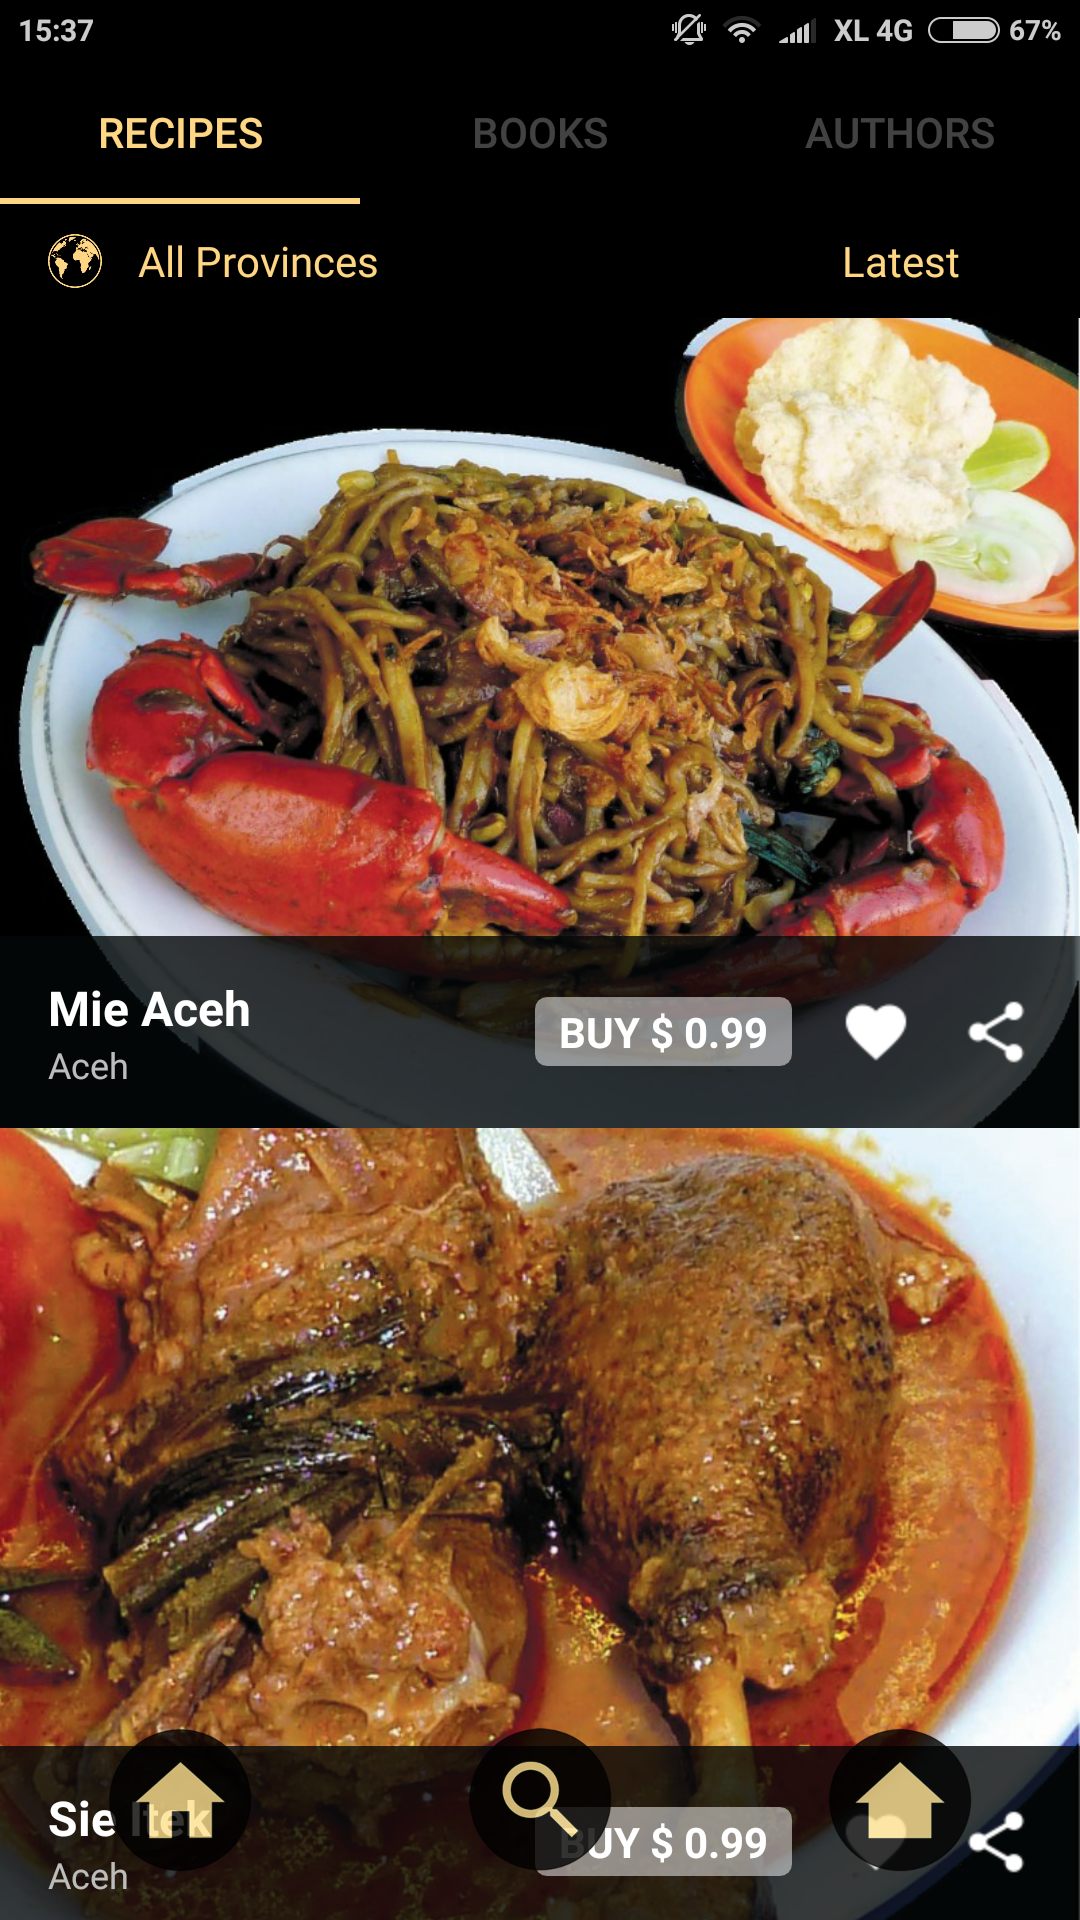
\includegraphics[width=0.3\textwidth]{gambar/kompas/utama}
	\caption{Halaman Utama Kompas Recipe}
\end{figure} 
\vspace{1cm}
Di dalam aplikasi tersebut terdapat kumpulan resep masakan yang dibagi menjadi dua jenis yaitu resep masakan berbayar dan resep masakan gratis. Terdapat banyak resep masakan yang menarik namun berbayar seperti Mie Aceh, Ayam Tangkap, dan Nasi Uduk. Untuk itu, penulis ingin mengembangkan aplikasi dengan resep masakan yang keseluruhannya gratis, sesuai dengan prinsip \textit{Open Source}.
\begin{figure}[H]
	\centering
	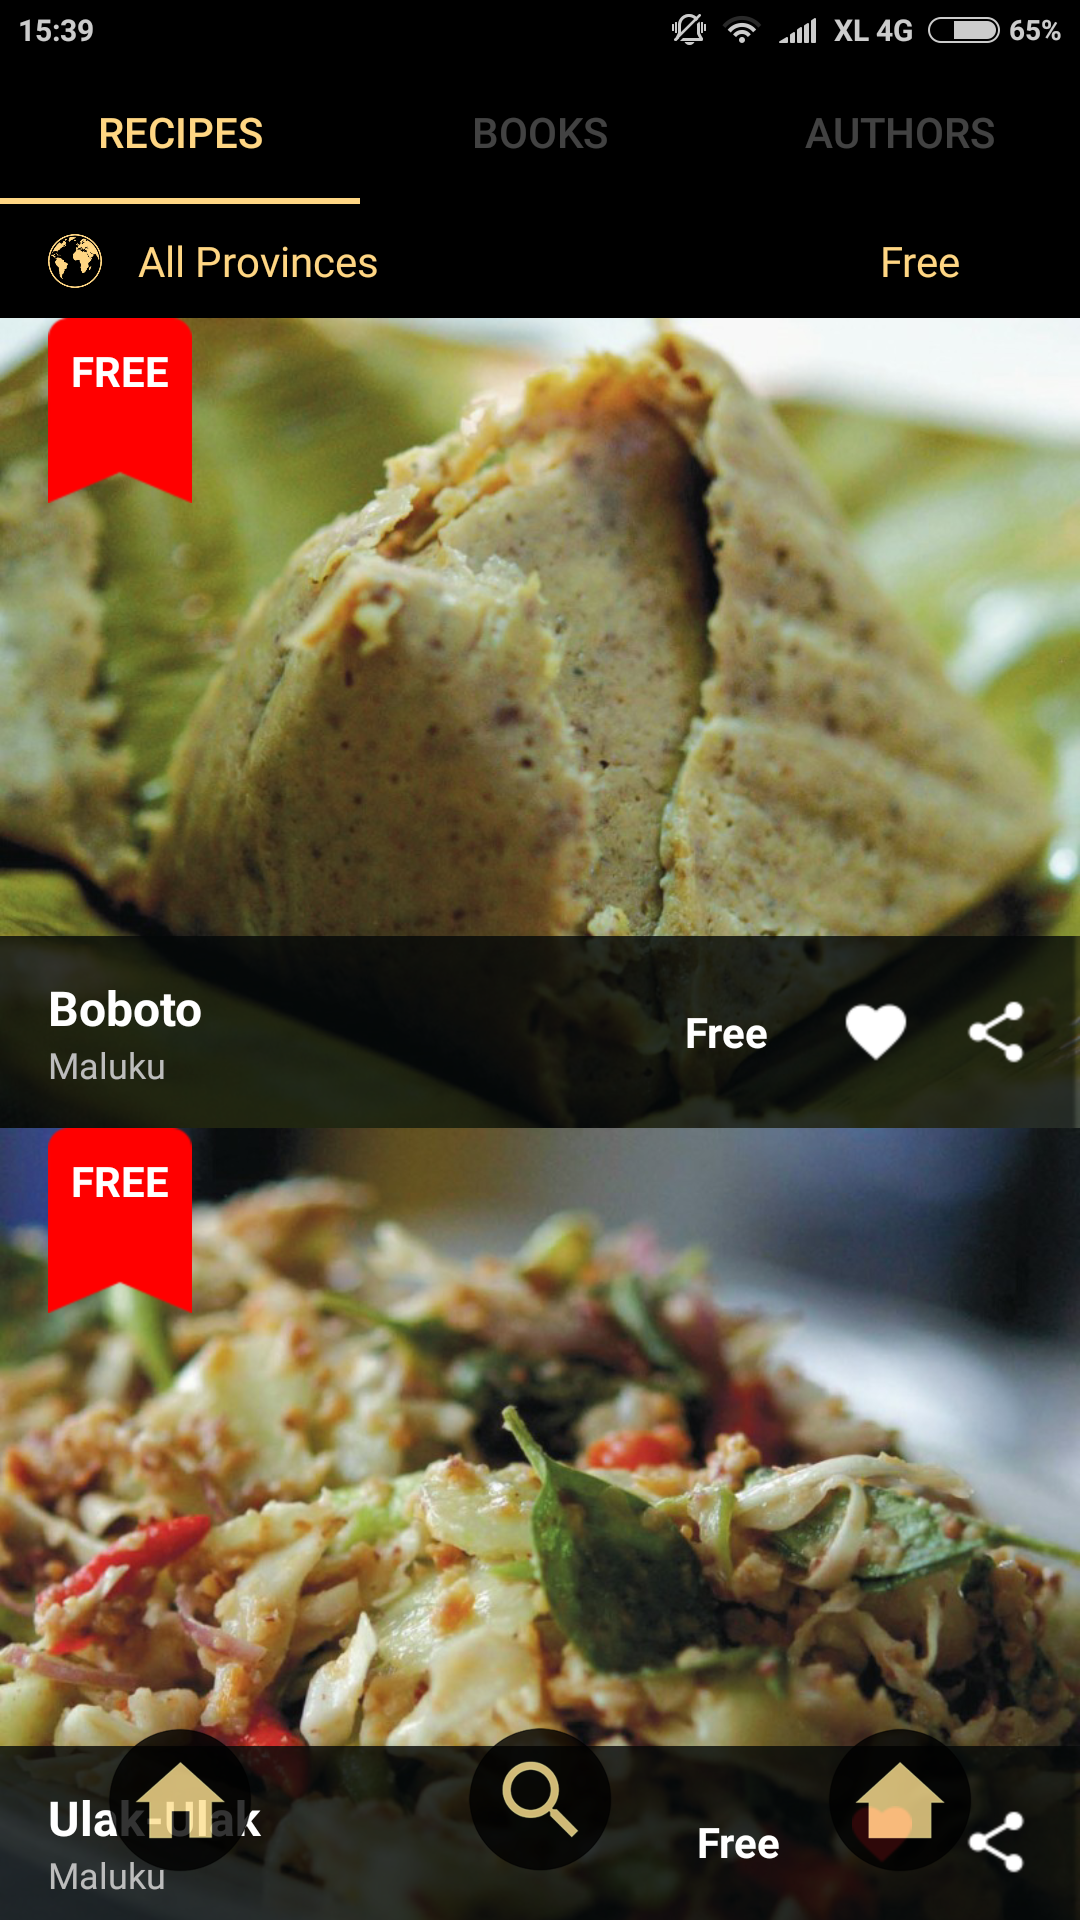
\includegraphics[width=0.3\textwidth]{gambar/kompas/free}
	\caption{Resep Masakan Gratis dari Kompas Recipe}
\end{figure} 
 Selain itu, Kompas Recipe tidak menyediakan video pembuatan makanan yang terdapat pada resep yang dibaca oleh pengguna. Aplikasi yang akan dibuat oleh penulis akan menyertakan video pembuatan makanan yang terdapat pada resep yang ada di dalam aplikasi tersebut. Penulis akan menamai aplikasi tersebut dengan nama Masak Yuk. Kata-kata tersebut sebenarnya merupakan ajakan bagi para masyarakat untuk memasak sendiri di rumah bersama keluarga, kerabat maupun teman-teman pengguna.


\section{Batasan Masalah}
Karena keterbatasan waktu, dana, tenaga, teori-teori dan supaya penelitian dapat dilakukan secara lebih mendalam maka tidak semua masalah akan diteliti. Berikut merupakan batasan-batasan yang diterapkan oleh peneliti
\begin{itemize}
	\item Peneliti akan membuat aplikasi tersebut dengan menggunakan \emph{software}  IDE (\emph{Integrated Development Environtment}) Android Studio. Peneliti memilih menggunakan Android Studio karena fiturnya yang sudah cukup lengkap dan sangat membantu dalam proses pembuatan aplikasi Android. Selain itu, kelengkapan API (\emph{Application Programming Interface}) dan banyaknya dukungan yang tersedia secara \emph{online} memudahkan peneliti dalam mengembangkan sebuah aplikasi Android.
	\item  Peneliti akan langsung menggunakan \emph{smartphone} berbasis Android dalam proses \emph{debugging} dan \emph{testing}. Versi android yang digunakan adalah Lollipop (Android 5.0) dengan API 21.
	\item Koneksi internet yang cepat, minimal pada kecepatan HSPA
	\item Banyaknya resep masakan yang akan dimasukkan kedalam aplikasi sejumlah 30 resep. Jumlah wishlist maksimal 3 resep.
	\item Uji coba hanya akan dilakukan oleh Ahli yang sudah berpartisipasi dalam proses identifikasi awal.
	\item Elemen-elemen yang akan diujikan pada uji coba ahli adalah konten, tampilan, dan fungsionalitas.
\end{itemize}
\vspace{1cm}
\section{Rumusan Masalah}
Rumusan masalah berdasarkan latar belakang di atas adalah:
\begin{enumerate}
	\item Bagaimanakah bentuk aplikasi resep masakan terintegrasi \emph{food channel} YouTube berbasis Android?
	\item Bagaimana cara mengembangkan aplikasi resep masakan terintegrasi \emph{food channel} YouTube berbasis Android?
	\item Bagaimana cara mengintegrasikan YouTube dengan aplikasi Android?
\end{enumerate}


\section{Tujuan Penelitian}
Tujuan dari penelitian ini adalah: 
\begin{enumerate}
	\item Untuk mengetahui bentuk atau wujud aplikasi resep masakan terintegrasi \emph{food channel} YouTube berbasis Android. 
	\item Untuk memaparkan fitur-fitur yang terdapat pada aplikasi tersebut. Selain itu, peneliti juga ingin menggali dan mengetahui cara mengembangkan aplikasi resep masakan terintegrasi food channel YouTube berbasis Android. 
	\item Untuk mengetahui lebih lanjut bagaimana cara mengintegrasikan YouTube, khususnya \emph{food channel} Youtube, dengan aplikasi Android. 
\end{enumerate}

\section{Manfaat Penelitian}
Penelitian ini memiliki banyak manfaat, yaitu: 
	\begin{enumerate}
		\item Bagi Penulis\\
		Melalui penulisan penelitian ini, penulis dapat memahami cara mengembangkan aplikasi Android secara baik dan benar serta mengetahui cara mengintegrasikan YouTube ke dalam sebuah aplikasi Android
		\item Bagi Program Studi Sistem Komputer\\
		Penulisan penelitian ini memberikan gambaran bagi seluruh mahasiswa khususnya bagig mahasiswa program studi Ilmu Komputer Universitas Negeri Jakarta tentang bagaimana cara mengembangkan suatu aplikasi Android yang tidak hanya bermanfaat bagi penulis saja tetapi juga bermanfaat untuk masyarakat dari berbagai kalangan, mulai dari anak-anak hingga orang dewasa yang ingin memasak dengan memanfaaatkan teknologi \emph{smartphone} Android sebagai referensi masakan mereka  
		\item Bagi Masyarakat\\
		Penelitian, termasuk aplikasi yag dibuat oleh penulis, dapat dimanfaatkan sebagai sumber referensi utama bagi masyarakat yang ingin memasak dan ingin memanfaatkan \emph{smartphone} sebagai media referensinya.  Menurut penulis, menggunaan \emph{smartphone} sebagai referensi memasak menggantikan buku resep adalah solusi praktis di era digital saat ini karena masyarakat tidak perlu lagi membeli buku atau membawa buku dalam jumlah yang banyak untuk memasak.		
	\end{enumerate}

\section{Jenis Penelitian}
Jenis Penelitian yang dijalani oleh Peneliti berjenis Rekayasa Produk. Jenis penelitian ini mengarahkan penulis kepada pengembangan sebuah sistem informasi berbasis aplikasi ponsel pintar \emph{smartphone}.		
% Baris ini digunakan untuk membantu dalam melakukan sitasi
% Karena diapit dengan comment, maka baris ini akan diabaikan
% oleh compiler LaTeX.
\begin{comment}
\bibliography{daftar-pustaka}
\end{comment}


%!TEX root = ./template-skripsi.tex
%-------------------------------------------------------------------------------
%                            BAB II
%               KAJIAN TEORI
%-------------------------------------------------------------------------------

\chapter{KAJIAN TEORI}                

Kumpulan resep masakan pada umumnya memuat berbagai macam makanan yang siap untuk dimasak. Makanan merupakan elemen penting yang membentuk suatu resep karena makanan adalah produk hasil akhir yang ingin dicapai melalui panduan yang terdapat dalam resep masakan. Resep masakan kemudian dijadikan konten utama dalam pengembangan yang dilakukan oleh penulis dengan menggunakan Android sebagai wadah bagi aplikasi atau perangkat lunak tersebut. Pengembangan resep masakan ini dilakukan berdasarkan tahapan \emph{System Development Life Cycle} (SDLC) yang berlaku secara umum dalam dunia \emph{software developing}.


\section{Pengembangan Aplikasi Perangkat Lunak}
	Pengembangan perangkat lunak pada umumnya sama dengan membangun sebuah gedung. Proses pertama dimulai dengan sebuah ide atau gagasan, lalu dilanjutkan dengan merubah ide atau gagasan tersebut menjadi sebuah desain sehingga dapat memberi gambaran lebih jelas tentang ide tersebut. Proses selanjutnya bersifat opsional, yakni melakuan revisi atau perubahan terhadap desain apabila dirasa tidak sesuai dengan yang diinginkan. Setelah itu, dilanjutkan dengan melakukan pembuatan cetak biru terhadap desain tersebut sehingga memperoleh gambaran yang lebih mendetail lagi dari masing-masing bagian gedung tersebut. Proses yang terakhir adalah membangun gedung tersebut berdasarkan cetak biru yang ada \cite{francis}. 
	
	Dalam proses pengembangan aplikasi perangkat lunak, terdapat istilah SDLC atau \emph{System Development Life Cycle}. SDLC adalah sebuah metode atau proses untuk memberikan pengertian bagaimana sebuah sistem informasi dapat mendukung kebutuhan bisnis dengan melakukan desain sebuah sistem, membangun sistem tersebut, dan mengimplementasikannya ke pengguna \cite{denis}.
	
	SDLC memiliki 4 tahapan utama yakni perencanaan, analisa, desain, dan implementasi. Dalam sebuah proyek pengembangan aplikasi perangkat lunak pastilah memiliki keempat tahapan tersebut, namun cara untuk melaksanakan tahapan-tahapan tersebut dapat berbeda-beda antara satu proyek dengan proyek lainnya. Setiap tahapan tersebut memiliki langkah-langkah tersendiri dalam menjalankan tahapan-tahapan tersebut sesuai dengan tujuan akhir dari masing-masing tahapan tersebut.
	
	\begin{figure}[H]
		\centering
		
\includegraphics[width=1\textwidth]{gambar/sdlc_overview}
		\caption{Empat Tahapan Utama SDLC}
		\label{sdlc_overview}
	\end{figure}
		
	Jenis-jenis pelaksanaan dari tahapan-tahapan SDLC terdiri dari \cite{pressman}:
	\begin{enumerate}
		\item \emph{Linear Process Flow}, yang mengeksekusi 4 tahapan tersebut secara berurutan
		\item \emph{Iterative Process Flow}, yang mengeksekusi secara berulang satu atau beberapa tahapan sebelum melanjutkan ke tahapan selanjutnya
		\item \emph{Evolutionary Process Flow}, mengeksekusi tahapan tersebut secara melingkar
		\item \emph{Parallel Process Flow}, mengeksekusi satuu atau beberapa tahapan secara bersamaan dengan tahapan lain. 
	\end{enumerate}

	Dalam metode SDLC terdapat beberapa model pengembangan yang dapat dijadikan acuan dasar kerangka kerja dalam proses pengembangan sebuah aplikasi perangkat lunak, yakni \emph{Waterfall Model}, \emph{Iterative Model}, \emph{Spiral Model}, \emph{V-Model}, \emph{Big Bang Model}, \emph{Agile Model}, \emph{Rapid Application Development (RAD) Model}, dan \emph{Prototyping Model}. Dalam pengembangan aplikasi resep masakan ini, penulis memilih menggunakan \emph{Spiral Model}.
	
	Model spiral memadukan sistematika dari pembangunan antara model iteratif (\emph{Iterative Model}) dengan aspek pengendalian dari model \emph{waterfall} (\emph{Waterfall Model}). Model spiral termasuk dalam jenis \emph{Evolutionary Process Flow}, yang mengeksekusi tahapan pengerjaan secara melingkar \cite{tutorialspoint}. Tahapan-tahapan yang akan dilakukan dalam penelitian ini mengikuti model pengembangan spiral, yaitu: \emph{Identification} (identifikasi kebutuhan), \emph{Design} (Desain Sistem), \emph{Construct and Build} (Pembuatan Sistem), dan \emph{Evaluation} (\emph{delivery feedback and release})
    \begin{figure}[H]
		\centering
		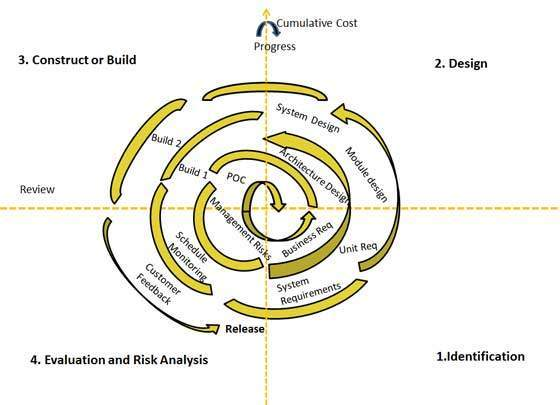
\includegraphics[width=0.6\textwidth]{gambar/sdlc_spiral_model}
		\caption{Model Spiral}
		\label{sdlc_spiral_model}
	\end{figure}

\section{\emph{Unified Modeling Language} (UML)}
	\emph{Unified Modeling Language} atau UML adalah sebuah Bahasa pemodelan terstandarisasi dan digunakan untuk berbagai kebutuhan dalam memodelkan pembuatan \emph{software}yang berorientasi pada obyek (\emph{object-oriented}). Standar tersebut dbuat dan dikelola oleh Object Management Group (OMG) pada tahun 1997 dan telah menjadi standar di bidang industri pembuatan \emph{software}. UML meliputi sebuah set dari teknik notasi grafis untuk membuat model dari sebuah sistem perangkat lunak berorientasi obyek secara visual. UML juga merupakan peralatan untuk menspesifikasikan dan memvisualisasikan sebuah sistem pada perangkat lunak. Hal tersebut mencakup tipe diagram yang telah terstandarisasi untuk mendeskripsikan serta memetakan sebuah aplikasi komputer atau desain serta struktur dari sebuah sistem basis data. UML memiliki fungsi untuk mengelola sistem yang besar dan kompleks. Memiliki struktur aplikasi yang jelas dapat membantu \emph{developer} dalam mengenalkan proyek kepada orang-orang baru maupun awam \cite{lee}.
	
	Jenis UML yang digunakan oleh peneliti pada pengembangan aplikasi ini adalah \emph{Use Case Diagram}, \emph{Class Diagram}, dan \emph{Activity Diagram}.
	
	\subsection{\emph{Use Case Diagram}}
		Fungsionalitas dari sebuah sistem basis data maupun sebuah perangkat lunak komputer dapat diilustrasikan dengan diagram \emph{use case}. Tugas utama dari sebuah \emph{use case} adalah memvisualisasikan kebutuhan fungsionalitas dari sebuah sistem, termasuk hubungan antara aktor (orang yang akan berinteraksi dengan sistem) dengan proses-proses yang esensial dalam sebuah sistem untuk mencapai suatu tujuan. Hal tersebut dapat dikategorikan sebagai kumpulan langkah-langkah yang mendefinisikan interaksi antara aktor dan sistem \cite{bell}.  
		
		\textit{Use Case Diagram} terdiri dari beberapa komponen, yakni:
		\begin{enumerate}
			\item Aktor\\ 
			Menggambarkan seorang aktor atau pengguna sistem yang akan berinteraksi dengan sistem
			\begin{figure}[H]
				\centering
				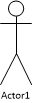
\includegraphics[width=0.05\textwidth]{gambar/use-case/aktor}
				\caption{Aktor dalam \textit{Use Case}}
			\end{figure}
			\vspace{1cm}
			\item Oval\\ 
			Bentuk Oval menggambarkan sistem yang dapat berinteraksi dengan aktor. Bentuk Oval tersebut biasanya disertai dengan nama aktivitas sistem di dalamnya yang terletak ditengah-tengah bentuk oval tersebut
			\begin{figure}[H]
				\centering
				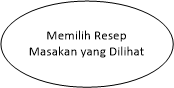
\includegraphics[width=0.4\textwidth]{gambar/use-case/balon}
				\caption{Sistem dengan Bentuk Oval}
			\end{figure}
		
			\item Garis Penghubung Aktor dan Sistem\\ 
			Untuk menggambarkan interaksi antara Aktor dan Sistem, diperlukan sebuah garis yang menghubungkan antara aktor dan sistem. Sebuah garis digunakan untuk menghubungkan keduanya
			\begin{figure}[H]
				\centering
				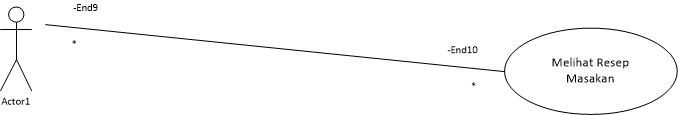
\includegraphics[width=0.8\textwidth]{gambar/use-case/penghubung_aktor_sistem}
				\caption{Garis Penghubungan antara Aktor dan Sistem}
			\end{figure}
			Melalui contoh di atas, dapat dilihat bahwa garis yang menyambungkan aktor dengan interaksi sistem menyatakan bahwa Aktor dapat Melihat Resep Masakan
			
			\item Garis Penghubung Antar Sistem\\ 
			Sistem yang terdapat pada \textit{use case} dapat berinteraksi satu sama lain. Terdapat dua jenis hubungan antar sistem, yakni \textit{include} dan \textit{extend}. Sesuai dengan namanya, \textit{include} menyatakan bahwa sebuah interaksi sistem yang terhubung adalah bagian dari interaksi sistem lainnya
			\begin{figure}[H]
				\centering
				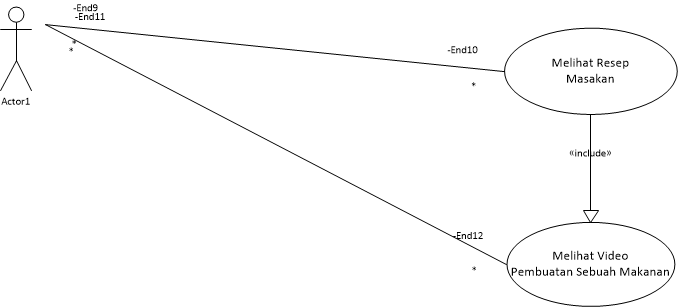
\includegraphics[width=0.8\textwidth]{gambar/use-case/include}
				\caption{Contoh Hubungan \textit{Include}}
			\end{figure}
			Contoh diatas menjelaskan bahwa Melihat Video Pembuatan Sebuah Makanan merupakan bagian dari Melihat  Resep Masakan. Sedangkan penghubung \textit{extend} menyatakan bahwa interaksi sebuah sistem merupakan perluasan dari interaksi sistem lainnya
			\begin{figure}[H]
				\centering
				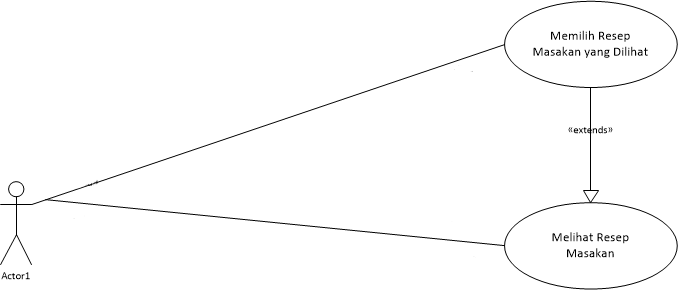
\includegraphics[width=0.8\textwidth]{gambar/use-case/extends}
				\caption{Contoh Hubungan \textit{Extend}}
			\end{figure}
			Contoh diatas menjelaskan bahwa Melihat Resep Masakan merupakan perluasan dari Memilih Resep Masakan yang Dilihat. Sebagai contoh, seorang Aktor dapat berinteraksi dengan sebuah sistem berbentuk aplikasi resep masakan. Interaksi yang dimungkinkan oleh sistem adalah Memilih Resep Masakan, Melihat Resep Masakan, dan Melihat Video Pembuatan Sebuah Resep Masakan. \textit{Use Case} dari interaksi tersebut terdapat pada Gambar \ref{use-case-example}.
			\begin{figure}[H]
				\centering
				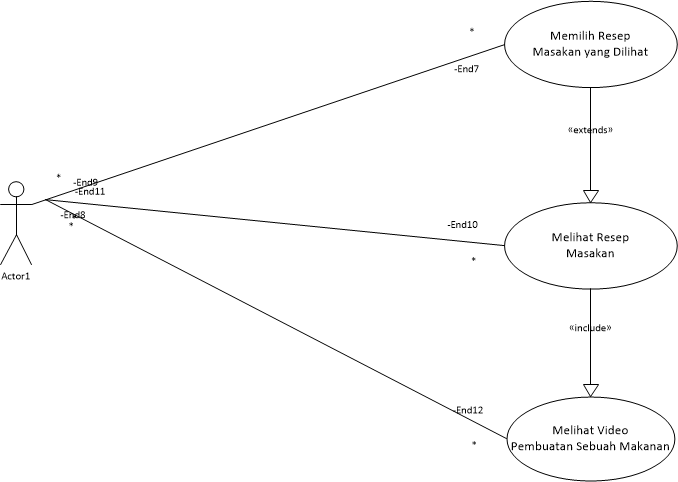
\includegraphics[width=1\textwidth]{gambar/use-case/contoh-use-case}
				\caption{Contoh \textit{Use Case} dalam Penggunaan Aplikasi Resep Masakan}
				\label{use-case-example}
			\end{figure}
			Jadi, dapat disimpulkan bahwa Use Case Diagram adalah sebuah diagram yang menggambarkan interaksi antara Aktor (pengguna) dengan sistem yang digunakan oleh Aktor.
			  

		\end{enumerate}
		
		
	\subsection{\emph{Class Diagram}}
		Struktur statis dari sebuah aplikasi komputer atau pangkalan basis data dapat digambarkan melalui sebuah \emph{class diagram}. \emph{Class diagram} juga menunjukkan perbedaan entitas (pengguna, alat, maupun data) yang berelasi satu sama lain. Diagram tersebut biasa digunakan untuk menampilkan class-class secara logikal, dan untuk mengimplementasikan class yang telah dibuat. \emph{Class diagram} merupakan unsur terpenting dalam pemodelan aplikasi berbasis obyek (\emph{object-oriented}) dan merupakan sebuah tipe struktur diagram statis yang mendeskripsikan struktur dari sebuah sistem dengan menampilkan \emph{class} dari sistem, atribut, operasi (method), dan relasi antar \emph{class} \cite{lee}.  
		
	\subsection{\emph{Activity Diagram}}
		Kontrol alur serta prosedur antara dua atau lebih obyek \emph{class} dalam memproses sebuah aktivitas dapat ditunjukkan melalui sebuah \emph{activity diagram}. Diagram tersebut dapat digunakan untuk memodelkan proses bisnis tingkat atas dalam sebuah level unit bisnis, atau untuk memodelkan aksi-aksi dalam class internal yang bersifat \emph{low level} (Bell, 2003). \emph{Activity Diagram} adalah representasi grafis dari sebuah alur pengerjaan yang berupa tahap-tahap dari berbagai aktivitas serta aksi dengan dukungan pilihan, iterasi, dan persetujuan. Pada UML, \emph{activity diagram} dapat digunakan untuk mendeskripsikan bisnis serta langkah-langkah operasional serta alur pengerjaan dari berbagai komponen yang berada dalam sebuah sistem. Sebuah \emph{activity diagram} menjelaskan keseluruhan alur dari sebuah sistem \cite{lee}. Contoh dibawah ini menjelaskan aktivitas pemrosesan pesanan dalam sebuah sistem Point of Sales (POS).  
		\begin{figure}[H]
			\centering
			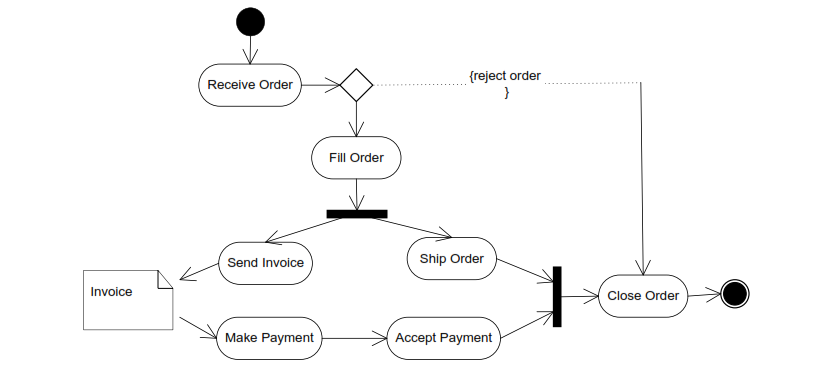
\includegraphics[width=1\textwidth]{gambar/sample-activity-diagram}
			\caption{Contoh \textit{Activity Diagram} dalam sistem Point Of Sales (POS)}
		\end{figure}
\section{\emph{Structured Query Language} (SQL)}
	SQL merupakan singkatan dari \emph{Structure Query Language}, didefinisikan sebagai suatu sintaks perintah-perintah tertentu atau bahasa program yang digunakan untuk mengelola suatu \emph{database} \cite{anisya}. SQL adalah sebuah konsep pengoperasian \emph{database}, terutama untuk pemilihan atau seleksi dan pemasukan data, yang memungkinkan pengoperasian data dikerjakan dengan mudah secara otomatis. Keandalan suatu sistem \emph{database} (DBMS) dapat diketahui dari cara kerja \emph{optimizer}-nya dalam melakukan proses perintah-perintah SQL, yang dibuat oleh user maupun program-program aplikasinya. 
	Query dikirimkan ke database dalam bentuk SQL Query Beberapa perintah yang umum digunakan adalah sebagai berikut:
	
	\begin{enumerate}
		\item 
		CREATE : Untuk membuat tabel baru
		\begin{figure}[H]
			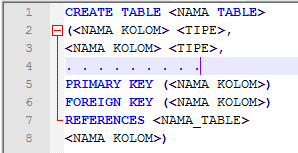
\includegraphics[width=0.4\textwidth]{gambar/sql/create}
		\end{figure}
		\item
		SELECT : Untuk mengambil \textit{record} dari database yang memenuhi kriteria tertentu
		\begin{figure}[H]
			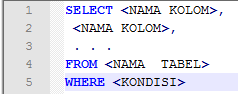
\includegraphics[width=0.5\textwidth]{gambar/sql/select}
		\end{figure} 
		\item
		INSERT : Untuk menambah \textit{record} ke dalam suatu tabel
		\begin{figure}[H]
			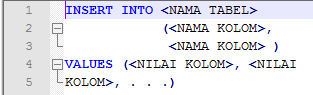
\includegraphics[width=0.5\textwidth]{gambar/sql/insert}
		\end{figure}
		\item
		UPDATE : Untuk merubah isi \textit{record} tertentu pada suatu tabel
		\begin{figure}[H]
			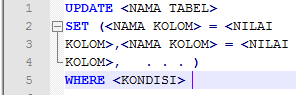
\includegraphics[width=0.5\textwidth]{gambar/sql/update}
		\end{figure}
		\item
		DELETE : Untuk menghapus \textit{record} pada suatu tabel
		\begin{figure}[H]
			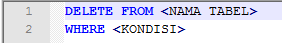
\includegraphics[width=0.5\textwidth]{gambar/sql/delete}
		\end{figure} 
		\item
		DROP : Untuk menghapus sebuah tabel
		\begin{figure}[H]
			
\includegraphics[width=0.5\textwidth]{gambar/sql/drop}
		\end{figure}
		\item
		JOIN : Untuk menggabungkan dua atau lebih tabel
		\begin{figure}[H]
			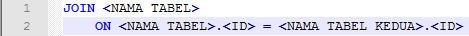
\includegraphics[width=0.8\textwidth]{gambar/sql/join}
		\end{figure}
	\end{enumerate}
		
\section{\emph{Entity Relationship Diagram} (ERD)}
	\emph{Entity Relationship Diagram} (ERD) adalah sekumpulan cara atau peralatan untuk mendeskripsikan data-data atau objek-objek yang dibuat berdasarkan dan berasal dari dunia nyata yang disebut entitas (\emph{entity}) serta relasi (\emph{relationship}) antar entitas-entitas tersebut dengan menggunakan beberapa notasi \cite{edi}. Komponen-komponen pembentuk ERD dapat di lihat pada Tabel \ref{tabel_komponen_erd}. 
	\begin{table}[H]
		\centering
		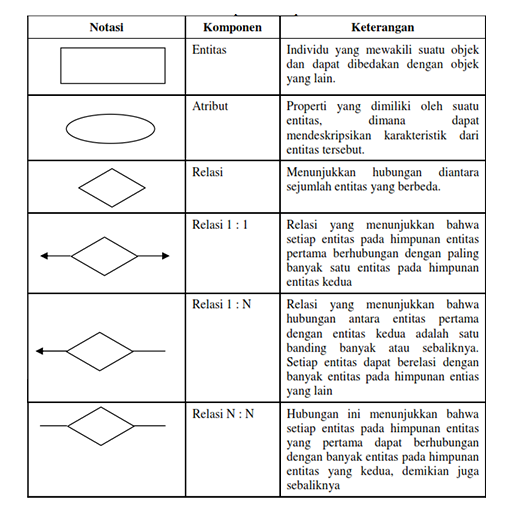
\includegraphics[width=0.8\textwidth]{gambar/erd/erd}
		\caption{Komponen-komponen Pembentuk ERD}
		\label{tabel_komponen_erd}
	\end{table}
	Sesuai dengan namanya, sebuah ERD memodelkan data sebagai entitas serta relasi (\emph{relationship}). Entitas adalah data yang ingin disimpan. Chen (1976) dalam presentasinya mendeskripsikan entitas sebagai  "sesuatu yang dapat diidentifikasi secara jelas." Jadi, entitas dapat berupa seseorang, sebuah tempat, obyek, kejadian, atau konsep yang ingin disimpan sebagai data. 
	
	Relasi (\emph{relationship}) adalah koneksi antara entitas-entitas yang ada. Relasi sendiri memiliki kardinalitas, yaitu ukuran kasar dari jumlah entitas (satu atau lebih) yang akan terkait dengan entitas lain (atau entitas). Berdasarkan kardinalitasnya, terdapat tiga jenis relasi yang dapat ditemukan dalam entitas-entitas yang ada yaitu relasi \emph{one-to-one} (1:1), \emph{one-to-many} (1:M), dan \emph{many-to-many} (M:N). Dalam relasi \emph{one-to-one}, sebuah entitas dapat berasosiasi dengan satu entitas lainnya dan sebaliknya. Contohnya, seorang siswa hanya memiliki satu sepeda. Dengan analogi antara siswa dengan sepeda tersebut, relasi \emph{one-to-many} menggambarkan bahwa seorang siswa dapat memiliki banyak sepeda. Sedangkan relasi \emph{many-to-many} pada analogi siswa dengan sepeda adalah banyak siswa yang dapat memiliki banyak sepeda dan sebaliknya \cite{bagui}. 
	
	Atribut adalah kategori dari sebuah data yang mendeskripsikan sebuah entitas atau relasi. Contoh dari atribut adalah sebuah entitas bernama MOBIL memiliki atribut tipe, warna, id\_kendaraan, dan lain sebagainya. Basis data sering digunakan untuk menyimpan data yang akan digunakan pada tahapan-tahapan selanjutnya. Sebuah atribut yang dapat digunakan untuk mencari suatu entitas tertentu disebut kunci atau \emph{key}. Atribut yang bersifat kunci (\emph{key}) dapat muncul secara natural apabila sebuah basis data dimodelkan dengan menggunakan ERD. Jika sebuah atribut dapat diperhitungkan menjadi sebuah ciri khas dari suatu entitas karena keunikannya, maka atribut tersebut disebut dengan \emph{candidate key} atau kandidat kunci. \emph{Candidate key} akan berubah menjadi \emph{primary key} apabila telah dipilih sebagai atribut khas suatu entitas yang bersifat paling unik daripada atribut lain yang terdapat pada suatu entitas.
	
	\subsection*{Studi Kasus Minimarket}
	Sebuah minimarket yang menjual berbagai jenis barang kebutuhan sehari-hari
	memiliki sebuah sistem informasi untuk mengelola penjualan secara langsung
	(point of sales), pengadaan barang, dan \textit{stock control}. Proses bisnis dalam penjualan barangnya dimulai pada saat \textit{customer} memilih barang yang akan dibeli. Setelah \textit{customer} memutuskan untuk membeli barang tersebut, maka kasir akan meminta informasi tentang identitas \textit{customer} untuk dicatat jika \textit{customer} yang bersangkutan terdaftar sebagai member. Namun jika \textit{customer} tersebut bukanlah member minimarket, maka data-data \textit{customer} akan diabaikan. Kemudian kasir akan membuatkan nota penjualan barang. Setelah barang diterima oleh \textit{customer}, \textit{customer} akan melakukan pembayaran. Proses berakhir ketika kasir memberikan bukti pembayaran kepada \textit{customer}. Sistem informasi yang tersedia tidak melayani proses pengembalian barang dan pemesanan barang. 
	Proses bisnis untuk pembelian barang dari supplier dimulai ketika pihak minimarket menghubungi supplier dan memesan barang. \textit{Supplier} kemudian akan membuatkan nota pembelian. Barang yang sudah dipesan lalu akan diantarkan ke minimarket.  Jika  barang  sudah  diterima,  maka  proses  yang  terjadi  adalah pembayaran dari pihak minimarket ke pihak \textit{supplier}. Setelah semua proses pembayaran  selesai,  \textit{supplier}  akan  memberikan  bukti  pembayaran  dan  proses selesai. Seperti halnya pada proses penjualan, proses pembelian tidak menangani pengembalian barang kepada \textit{supplier}. 
	Untuk proses \textit{stock control}, dilakukan proses pencatatan terhadap barang yang di- supply, barang yang dibeli oleh \textit{customer} dan sisa barang yang ada di gudang per harinya. Hal ini dimaksudkan agar setiap keluar masuknya barang yang ada dapat terawasi dan menjaga barang selalu tersedia di gudang. 
	Maka ERD yang dapat dibuat dari kasus diatas adalah sebagai berikut:
	\begin{figure}[H]
		\centering
		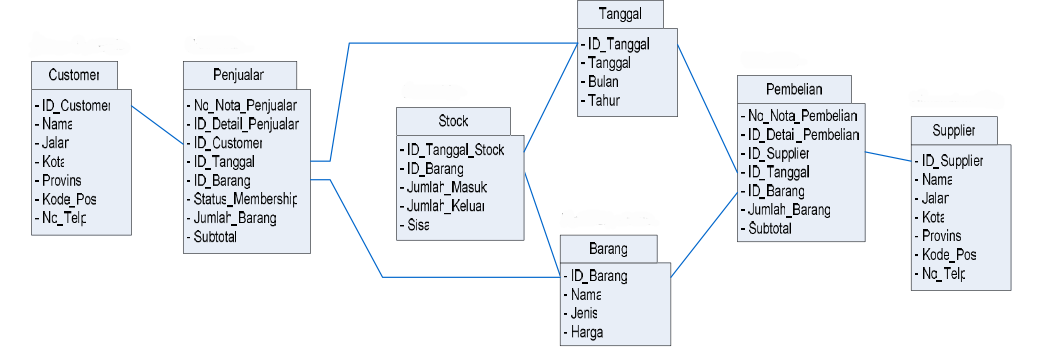
\includegraphics[width=1.1\textwidth]{gambar/erd/sample-erd}
		\caption{ERD Studi Kasus Minimarket}
	\end{figure}
	
	
	
\section{Pengertian Android}
	Android adalah sebuah sistem operasi untuk perangkat \emph{mobile} berbasis linux yang mencakup sistem operasi, \emph{middleware} dan aplikasi. Android menyediakan \emph{platform} terbuka bagi para pengembang untuk menciptakan aplikasi mereka \cite{murtiwiyati}. Dikutip dari situs resmi Open Handset Alliance, yang merupakan pengembang sistem operasi Android pertama di dunia, Android dikembangkan untuk memungkinkan para pengembang aplikasi membuat suatu aplikasi \emph{mobile} yang dapat memanfaatkan seluruh kelebihan yang ditawarkan dari suatu perangkat \emph{mobile}. Android dibuat secara terbuka dan semua orang dapat mengembangkan dan menggunakan semua fungsionalitasnya. Contohnya, sebuah aplikasi yang dapat digunakan untuk melakukan berbagai macam fungsionalitas sebuah ponsel seperti membuat panggilan, mengirimkan pesan singkat, atau mengambil gambar dengan kamera, memungkinkan para pengembang aplikasi untuk membuat banyak sekali fitur lainnya yang dapat digunakan oleh para penggunanya. Android dibuat dengan menggunakan Kernel Linux yang bersifat terbuka (\emph{open source}). Selain itu, Android juga merupakan hasil dari modifikasi mesin virtual (\emph{virtual machine}) yang didesain untuk mengoptimalkan memori serta perangkat keras (\emph{hardware}) pada sebuah ponsel. Android sendiri adalah open source yang berarti dapat terus dikembangkan menjadi sebuah teknologi baru sesuai dengan kebutuhan manusia pada saat ini. \emph{Platform} ini akan terus berkembang seiring dengan pergerakan para pengembang aplikasi yang bekerja bersama-sama untuk membangun aplikasi \emph{mobile} yang inovatif. 
	
	Gambar \ref{android-sbg-platform} menunjukkan hirarki aplikasi yang dibuat oleh peneliti terhadap \textit{platform} Android.   
	
	\begin{figure}[H]
		\centering
		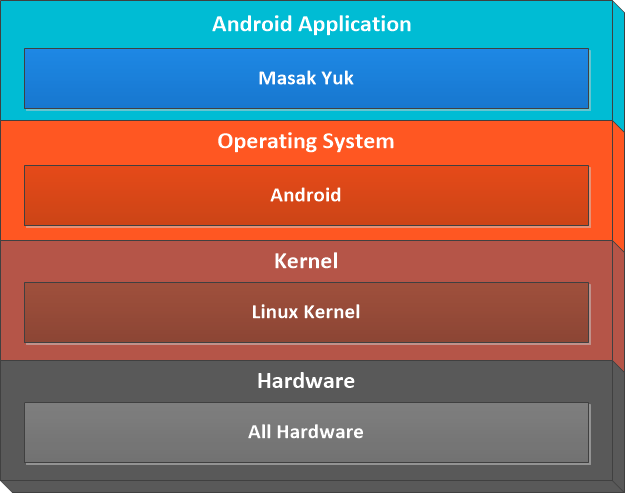
\includegraphics[width=1\textwidth]{gambar/stack-diagram-bab-2}
		\caption{\textit{Stack Diagram} Hirarki Aplikasi Android dengan Komponen Lainnya}
		\label{android-sbg-platform}
	\end{figure}
	

	Selain kemampuannya untuk mendukung dan memfasilitasi berbagai fungsi familiar seperti membuat panggilan, berkirim pesan elektronik, dan mencari sebuah restoran, perangkat Android dapat menjadi sebuah perangkat dengan fungsi tanpa batas dan dapat dikembangkan kapan saja bergantung pada pemikiran para pengembangnya \cite{rogers}. Saat ini, Android tidak hanya terdapat pada sebuah ponsel tetapi juga tertanam dalam sebuah tablet, televisi, kacamata pintar, kulkas, mobil dan lain sebagainya. Jadi dapat disimpulkan bahwa Android merupakan sistem operasi untuk sebuah perangkat cerdas yang dapat memiliki banyak fitur dan fungsi sesuai dengan keinginan para pengembangnya untuk menjawab masalah-masalah yang terdapat dalam kehidupan manusia. 

\section{Android Studio}
	Android Studio merupakan sebuah \emph{Integrated Developing Environment} (IDE) untuk \emph{platform} Android. Android Studio ini diumumkan pada tanggal 16 Mei 2013 pada konferensi Google I/O oleh \emph{Product Manager} Google, Ellie Powers. Android Studio bersifat \emph{free} dibawah Apache \emph{License} 2.0. Versi awal Android Studio yaitu 0.1 dirilis pada bulan Mei 2013. Kemudian dibuat versi \emph{beta} 0.8 yang dirilis pada bulan Juni 2014. Versi yang paling stabil dirilis pada bulan Desember 2014, dimulai dari versi 1.0. Berbasiskan JetBrainns' IntelliJ IDEA, Studio di desain khusus untuk Android \emph{Development}. Android Studio sudah bisa diunduh untuk Windows, Mac OS X, dan Linux

	Berikut ini adalah beberapa keunggulan Android Studio:
	\begin{enumerate}
		\item Android \emph{Memory} (HPROF) \emph{Viewer}\\
		Android Studio kini mengizinkan penggunanya untuk menangkap dan menganalisa \emph{snapshot} memori dalam format Android HPROF.
		\item \emph{Allocation Tracker}\\
		Untuk mempermudah dalam menganalisa penggunaan alokasi memori aplikasi yang dibuat oleh penggunanya, \emph{Allocation Tracker} kini menambahkan fitur visual. Dengan adanya fitur ini, alokasi memori yang digunakan oleh aplikasi yang dibuat oleh penggunanya dapat terlihat dalam diagram berbentuk lingkaran.
		\item APK \emph{Test}\\
		Kini plugin baru ('com.android.test') telah ditambahkan untuk mempermudah penggunanya dalam mencoba atau melakukan \emph{testing} aplikasi Android yang sedang dikembangkan. Untuk menggunakan fitur ini, penggunanya harus memiliki Gradle Plugin versi 1.3.
		\item \emph{Application Permission Annotation}\\
		Android Studio (sejak versi 1.3) mendukung \emph{inline code annotation} yang akan membantu penggunanya mengatur \emph{app permission} yang dirilis pada Android M (Android 6.0/Marshmallow).
		\item SDK \emph{Auto Update} dan SDK \emph{Manager}
		Android Studio mengatur pembaharuan SDK dan plugin-plugin lainnya secara otomatis.
	\end{enumerate}

\section{\emph{Application Programming Interface} (API)}
	\emph{Application Programming Interfaces} atau biasa disingkat API, yang didalamnya termasuk kumpulan \emph{library}, \emph{framework}, peralatan penunjang (\emph{toolkits}), dan peralatan pengembangan \emph{software} lainnya, digunakan secara virtual dalam semua bahasa pemrograman \cite{myers}. Jika sebuah perangkat lunak mengandung API \emph{internal} (yang berasal dari dalam perangkat lunak tersebut) serta API publik (seperti Java Platform SDK, Windows .NET Framework, jQuery untuk JavaScript, dan Web services seperti Google Map), maka setiap baris dari kode yang ditulis oleh \emph{programmer} memanggil dan menggunakan API. API menyediakan sebuah mekanisme dalam penggunaan kembali sebuah kode yang telah dibuat sebelumnya sehingga \emph{programmer} dapat memanfaatkannya kembali untuk keperluan yang berbeda. Hal ini sangat efektif apabila dibandingkan dengan membuat setiap program dan kode dari awal. Lebih lanjut lagi, penggunaan API sangat dibutuhkan karena akses yang bersifat \emph{low-level} menuju kepada sebuah sumber dari suatu sistem (seperti grafik atau gambar, \emph{networking}, dan \emph{file} sistem) yang tersedia hanya melalui API yang terproteksi.
	
	\begin{figure}[H]
		\centering
		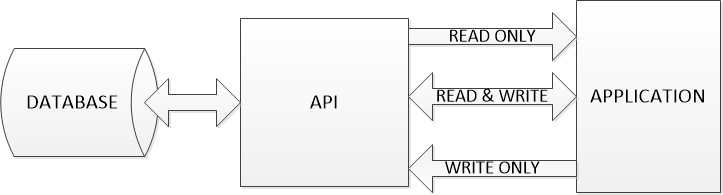
\includegraphics[width=1\textwidth]{gambar/api/api_chart}
		\caption{Cara Kerja API}
	\end{figure}

	API menjembatani sebuah basis data dengan aplikasi yang mengakses basis data tersebut. Terdapat tiga jenis metode yang dihasilkan oleh API, yaitu metode \textit{read only} (hanya membaca), \textit{write only} (menulis atau mengubah saja), dan \textit{read and write} (membaca dan menulis atau mengubah data). Ketiga jenis metode tersebut dibuat sesuai dengan kebutuhan aplikasi yang akan dijembatani oleh API.   
	 
	
\section{Integrasi YouTube dengan Aplikasi Android}
	YouTube dapat diintegrasikan ke dalam sebuah aplikasi Android dengan mengimplementasikan API (\emph{Application Programming Interface}) yang disediakan oleh YouTube dan Google secara gratis (\emph{open source}) yang berarti semua orang dapat menggunakannya tanpa terkecuali. API tersebut dinamakan YouTube Android Player API.
	
	Dilansir dari situs Google Developer, API tersebut memungkinkan penggunanya untuk memasukkan fungsi pemutaran video ke dalam aplikasi Android. API tersebut mendefinisikan metode untuk menampilkan dan memainkan video-video YouTube (dan juga \emph{playlist}) dan untuk memodifikasi serta mengatur pemutaran video dalam aplikasi Android.
	
	\begin{figure}[H]
		\centering
		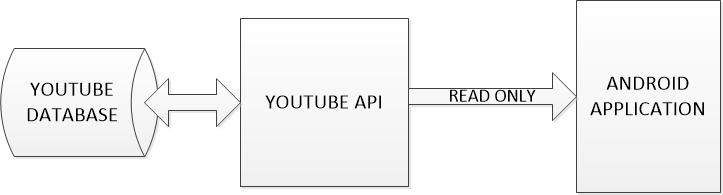
\includegraphics[width=1\textwidth]{gambar/api/youtube_api_chart}
		\caption{Cara Kerja YouTube API}
	\end{figure}

	YouTube Android Player API termasuk dalam jenis API yang menyediakan \textit{read only method}, yaitu API yang menyediakan metode untuk membaca data yang terdapat dalam sebuah basis data, dimana basis data yang digunakan pada aplikasi ini adalah basis data YouTube. Video dialirkan kedalam aplikasi Android menggunakan berbagai macam metode yang terdapat dalam API YouTube tersebut. 
	
	Dengan menggunakan API tersebut, pengguna dapat menampilkan berbagai video ke dalam sebuah pemutar yang terintegrasi pada \emph{User Interface} (UI) penggunanya. Kemudian penggunanya juga dapat mengatur pemutaran video secara terprogram. Sebagai contoh, pengguna dapat memainkan, melakukan jeda, atau mempercepat video ke titik tertentu pada video yang sedang diputar
	
	Pengguna juga dapat memasukkan \emph{event listener} untuk mendapatkan \emph{callbacks} dari beberapa event, seperti pemuatan video pada pemutar video atau perubahan tahap pada pemutar video. Dan yang terakhir, API tersebut memiliki \emph{helper functionality} (fungsionalitas pembantu) untuk mendukung perubahan orientasi seperti transisi menjadi pemutaran dalam layar penuh (\emph{fullscreen playback}).
	
	Langkah-langkah untuk menginisialisasi integrasi YouTube dengan aplikasi Android:
	\begin{enumerate}
		\item Unduh terlebih dahulu file YouTube Android Player API pada link 
		\url{https://developers.google.com/youtube/android/player/downloads/}
		\begin{figure}[H]
			\centering
			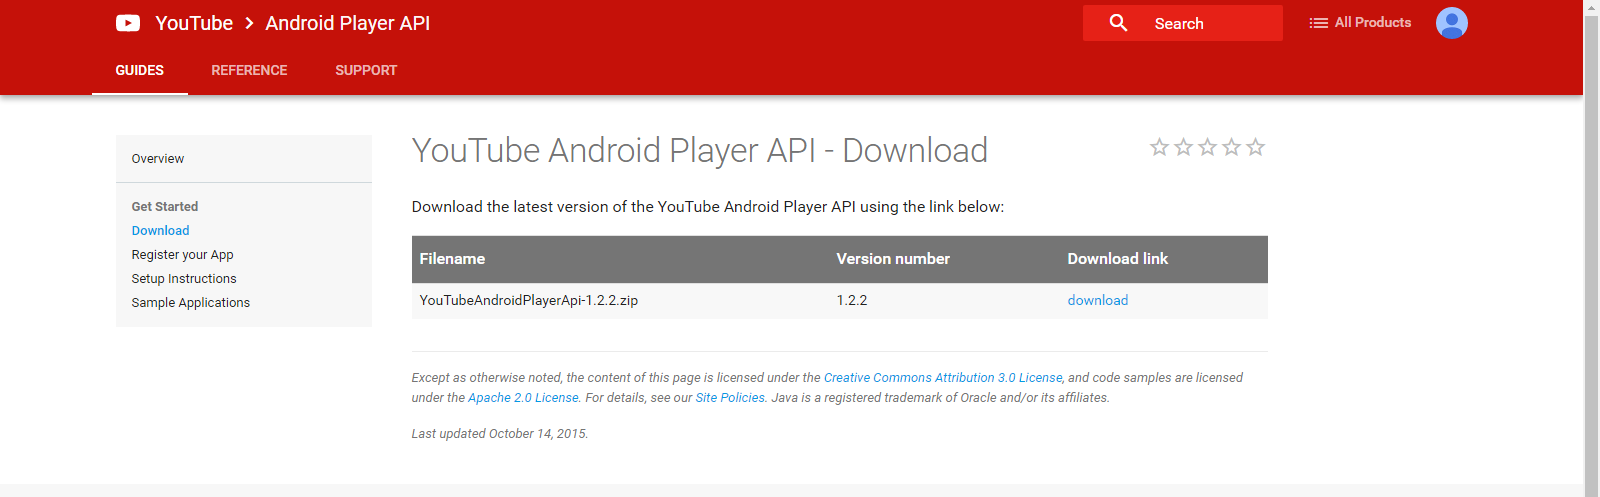
\includegraphics[width=1\textwidth]{gambar/y0}
			\caption{Laman Unduh YouTube Player Android API}
		\end{figure}
		
		\item Kemudian pada Android Studio, ubah tampilan \textit{tree} dari Android menjadi Project dan buat direktori baru bernama \textit{libs} pada direktori \textit{app}
		\begin{figure}[H]
			\centering
			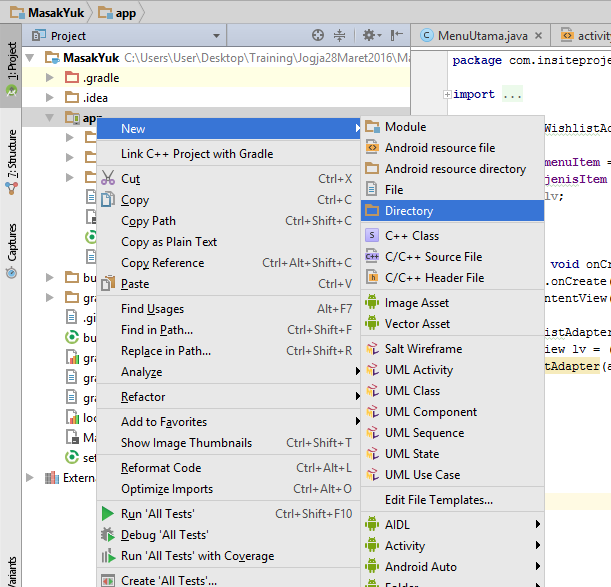
\includegraphics[width=0.8\textwidth]{gambar/y2}
			\caption{Tampilan \textit{tree} Project}
		\end{figure}
		
		\item Ekstrak berkas yang telah diunduh pada langkah pertama dan salin 
		berkas YouTubeAndroidPlayerApi.jar pada direktori \textit{libs}
		\begin{figure}[H]
			\centering
			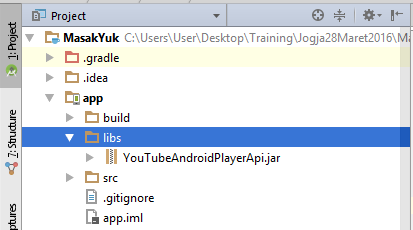
\includegraphics[width=1\textwidth]{gambar/y3}
			\caption{Menyalin Berkas YouTube API}
		\end{figure}	
		
		\item Tambahkan kode compile files('libs/YouTubeAndroidPlayerApi.jar') pada berkas build.gradle yang terdapat di dalam direktori \textit{app}
		\begin{figure}[H]
			\centering
			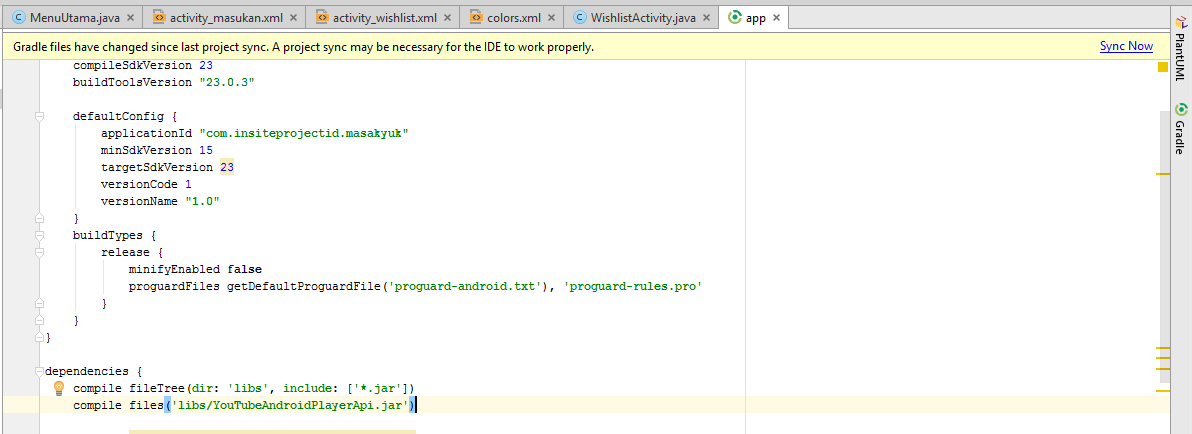
\includegraphics[width=1\textwidth]{gambar/y4}
			\caption{Menambah Baris Kode}
		\end{figure}
	
		\item Akan muncul sebuah pemberitahuan untuk melakukan sinkronisasi pustaka yang ada dengan pustaka YouTube API. Klik \textit{Sync Now} pada pemberitahuan tersebut untuk menginisialisasikan Android dengan YouTube
		\begin{figure}[H]
			\centering
			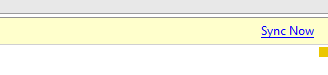
\includegraphics[width=1\textwidth]{gambar/y5}
			\caption{\textit{Sync Now}}
		\end{figure}
		
		\item Buat sebuah Activity dan tambahkan baris kode yang sama dengan kode yang tertera di bawah ini 
		\begin{figure}[H]
			\centering
			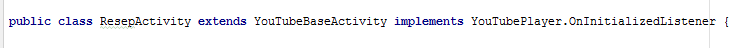
\includegraphics[width=1\textwidth]{gambar/y6}
			\caption{Menambah Baris Kode pada Activity}
		\end{figure}
		
		\item Inisialisasikan YouTubePlayerView pada Activity tersebut
		\begin{figure}[H]
			\centering
			
\includegraphics[width=0.6\textwidth]{gambar/y7}
			\caption{Inisialisasi YouTubePlayerView}
		\end{figure}
	
		\item Inisialisasikan juga YouTubePlayerView yang sudah disiapkan pada Activity tersebut ke dalam \textit{method} onCreate.
		\begin{figure}[H]
			\centering
			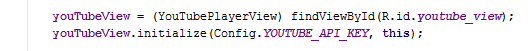
\includegraphics[width=1\textwidth]{gambar/y8}
			\caption{Inisialisasi YouTubePlayerView ke dalam \textit{method} onCreate}
		\end{figure}
		
		\item Pada \textit{layout}, tambahkan baris kode di bawah ini untuk menginisialisasi tampilan YouTube
		\begin{figure}[H]
			\centering
			
\includegraphics[width=1\textwidth]{gambar/y9}
			\caption{Inisialisasi Tampilan YouTube}
		\end{figure}
		
		\item Implementasikan \textit{method} yang berasal dari API YouTube dengan melakukan klik pada lampu merah yang terdapat pada inisialisasi \textit{class} Activity seperti yang terdapat di bawah ini
		\begin{figure}[H]
			\centering
			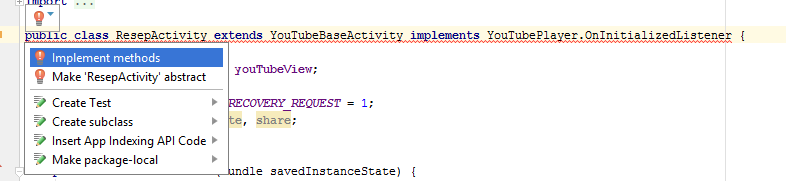
\includegraphics[width=1\textwidth]{gambar/y10-a}
			\caption{Implementasi \textit{Method} YouTube}
		\end{figure}
	
		\item Akan muncul dua \textit{method} penting dalam mengintegrasikan YouTube ke dalam Android, yaitu onInitializationSuccess dan onInitializationFailure seperti di bawah ini 
		\begin{figure}[H]
			\centering
			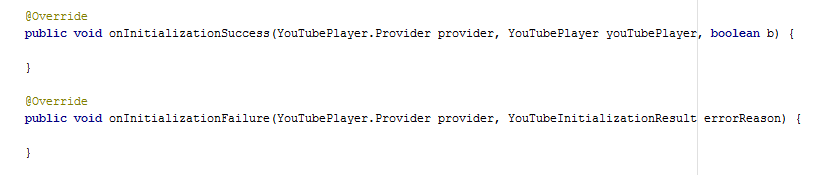
\includegraphics[width=1\textwidth]{gambar/y10}
			\caption{Inisialisasi Tampilan YouTube}
		\end{figure}
		onInitializationSuccess adalah method yang berfungsi untuk menjalankan fitur-fitur YouTube di dalam aplikasi Android apabila inisialisasi sukses. Sedangkan onInitializationFailure adalah metode untuk mengambil alih tindakan yang terjadi apabila YouTube gagal diinisialisasikan.
		
		\item Untuk memutar sebuah video YouTube, API membutuhkan masukan berupa karakter alfanumerik yang terdapat pada akhir dari link YouTube.
		\begin{figure}[H]
			\centering
			
\includegraphics[width=1\textwidth]{gambar/y12}
			\caption{Contoh Karakter Alfanumerik YouTube}
		\end{figure}
		
		Berikut adalah contoh pengaplikasiannya
		\begin{figure}[H]
			\centering
			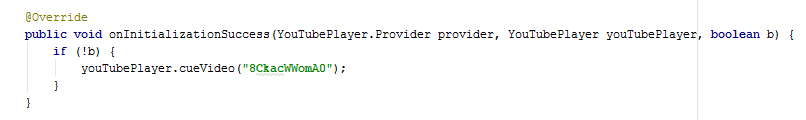
\includegraphics[width=1\textwidth]{gambar/y11}
			\caption{Contoh Pengaplikasian Karakter Alfanumerik YouTube}
		\end{figure}
		
	\end{enumerate}
		
	
	API \emph{client library} berinteraksi dengan sebuah layanan yang terdistribusi sebagai sebuah bagian dari aplikasi YouTube untuk platform Android. \emph{Client library} tersebut meninggalkan sedikit jejak kaki, dengan kata lain tidak akan membebani atau menjadikan ukuran file aplikasi menjadi lebih besar
	


% Baris ini digunakan untuk membantu dalam melakukan sitasi
% Karena diapit dengan comment, maka baris ini akan diabaikan
% oleh compiler LaTeX.
\begin{comment}
\bibliography{daftar-pustaka}
\end{comment}


%!TEX root = ./template-skripsi.tex
%-------------------------------------------------------------------------------
%                            BAB III
%               		PEMBAHASAN
%-------------------------------------------------------------------------------

\chapter{IMPLEMENTASI PROGRAM}

Sesuai dengan tahapan-tahapan pengembangan perangkat lunak yang tertera pada SDLC, maka penulis melakukan serangkaian kegiatan untuk menunjang pengembangan aplikasi resep masakan berbasis Android ini. Karena menggunakan SDLC Model Spiral, maka penulis akan melakukan beberapa tahapan yaitu identifikasi, desain, konstruksi dan pembangunan, serta evaluasi. Evaluasi akan dibahas pada Bab IV (Uji Coba dan Hasil Percobaan) Adapun alur dari aplikasi yang akan dibuat dijelaskan pada Gambar \ref{alur_app}

\begin{figure}[H]
	\centering
	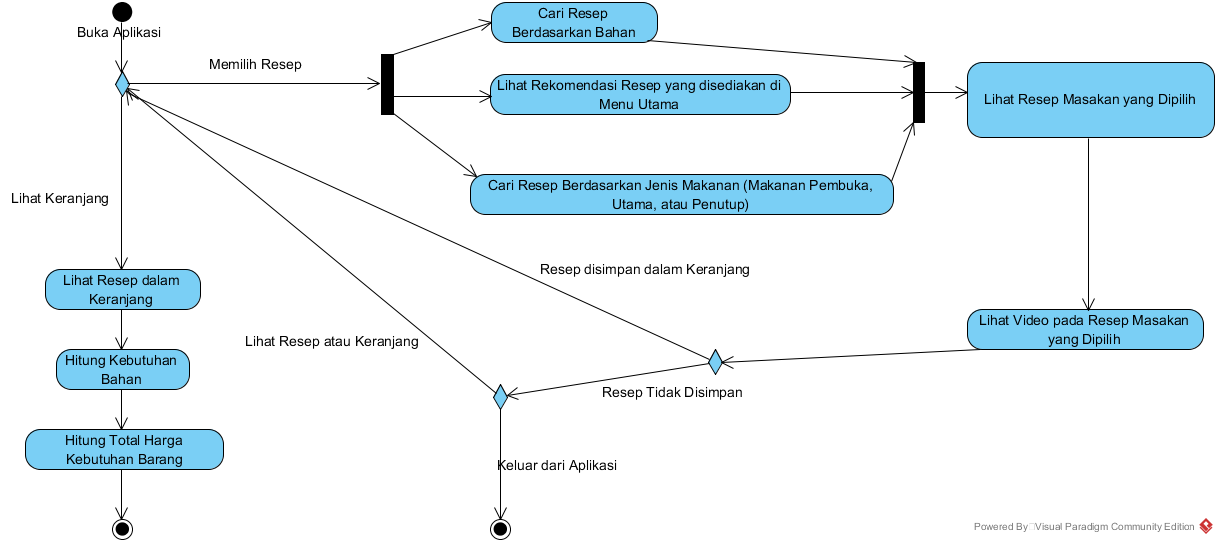
\includegraphics[width=1\textwidth]{gambar/activity_diagram_v2}
	\caption{Alur Kerja Aplikasi}
	\label{alur_app}
\end{figure}


\section{Identifikasi}
	Penulis mengumpulkan beberapa informasi yang dibutuhkan untuk membangun aplikasi ini dengan cara menyebarkan beberapa kuisioner kepada ahli di bidang masakan, baik itu chef, asisten chef, serta pemilik usaha dibidang kuliner untuk mengetahui fitur apa sajakah yang seharusnya ada dalam aplikasi berbasis Android ini. Penulis juga tidak lupa meminta pandangan kepada beberapa kaum awam yang berasal dari berbagai kalangan untuk mengetahui tentang pendapat masyarakat tentang fitur apa saja yang seharusnya terdapat pada aplikasi resep masakan ini. 
	
	Dari 4 responden yang merupakan para ahli, dimana 2 dari 4 responden tersebut adalah chef, satu orang asisten chef, dan seorang pemilik usaha kuliner, fitur menampilkan banyak resep masakan sekaligus merupakan fitur yang paling banyak dipilih dengan nilai 2. Sedangkan fitur lain yang diusulkan penulis seperti menampilkan sebuah resep makanan, menyimpan beberapa resep masakan sekaligus kedalam sebuah troli untuk dibuat dalam jangka waktu tertentu, menghitung total kebutuhan bahan untuk dua resep atau lebih sekaligus, serta menghitung total harga yang dibutuhkan untuk membeli bahan-bahan masakan mendapatkan masing-masing nilai 1.
	
	\begin{figure}[H]
		\centering
		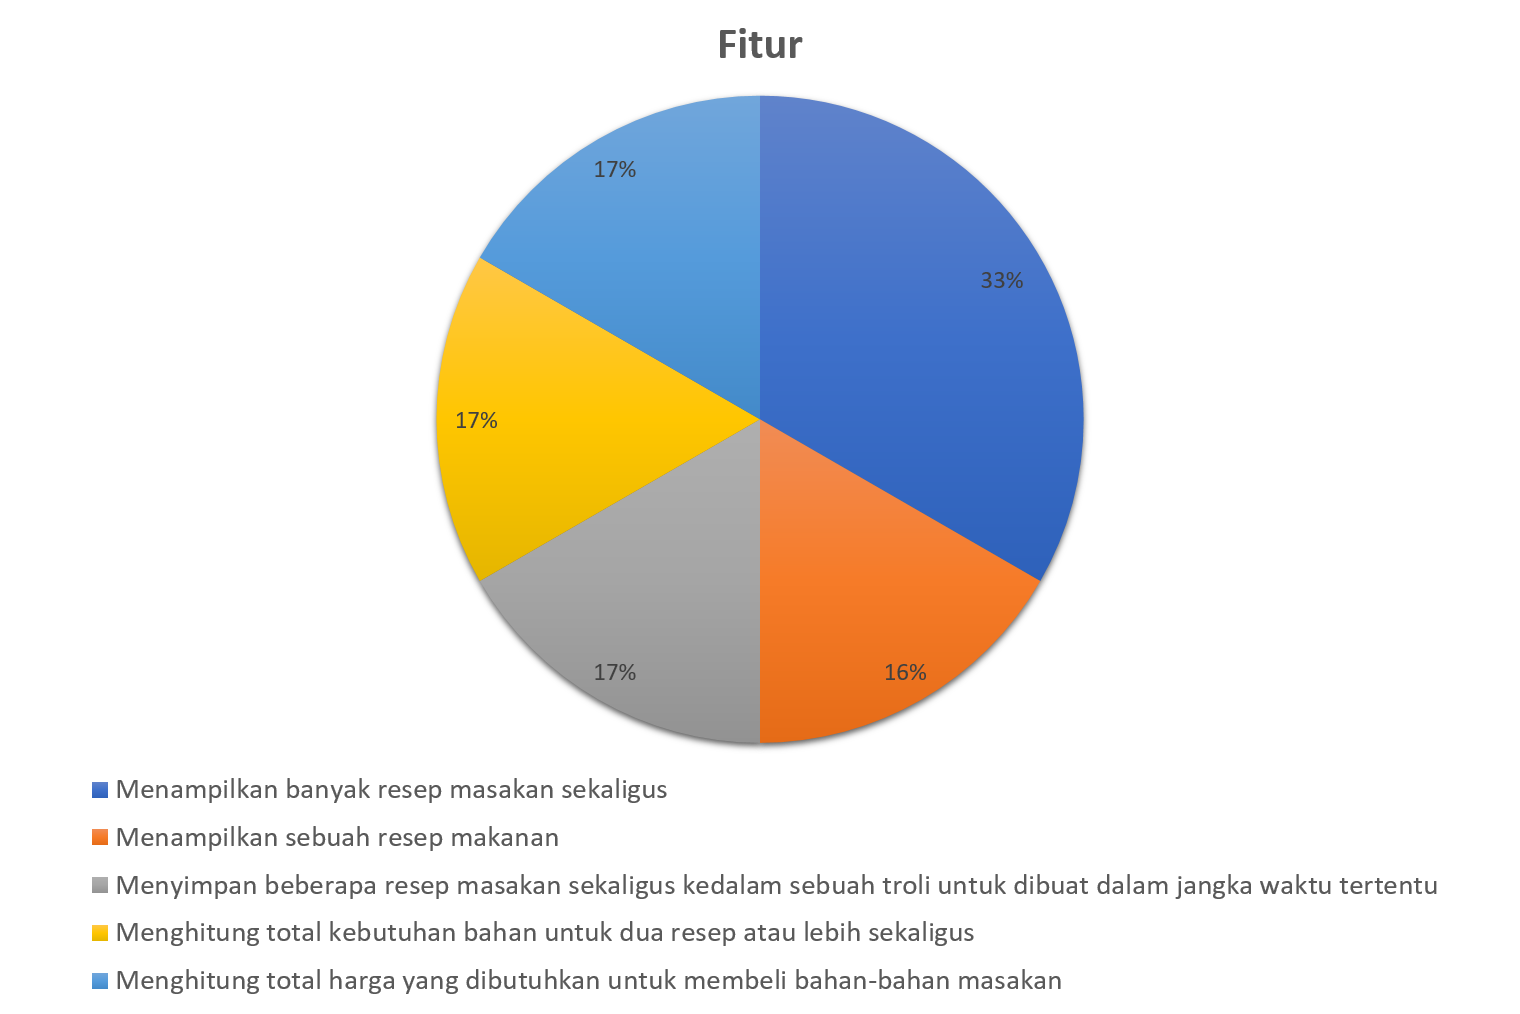
\includegraphics[width=1\textwidth]{gambar/pie/kuisioner_ahli}
		\caption{\textit{Pie Chart} Hasil Kuisioner Ahli}
	\end{figure}
	
	Untuk responden yang berasal dari kaum awam yang berjumlah 9 orang, dimana 2 dari 9 orang responden berprofesi sebagai guru, satu orang berprofesi sebagai ibu rumah tangga, sedangkan sisanya adalah seorang karyawan swasta, fitur menampilkan banyak resep masakan sekaligus merupakan fitur yang paling banyak dipilih dengan nilai 7. Sementara fitur menghitung total kebutuhan bahan untuk dua resep atau lebih sekaligus berada pada peringkat 2 dengan nilai 3. Sedangkan fitur lain yang diusulkan penulis seperti menampilkan sebuah resep makanan, menyimpan beberapa resep masakan sekaligus kedalam sebuah troli untuk dibuat dalam jangka waktu tertentu, serta menghitung total harga yang dibutuhkan untuk membeli bahan-bahan masakan mendapatkan masing-masing nilai 2.
	
	\begin{figure}[H]
		\centering
		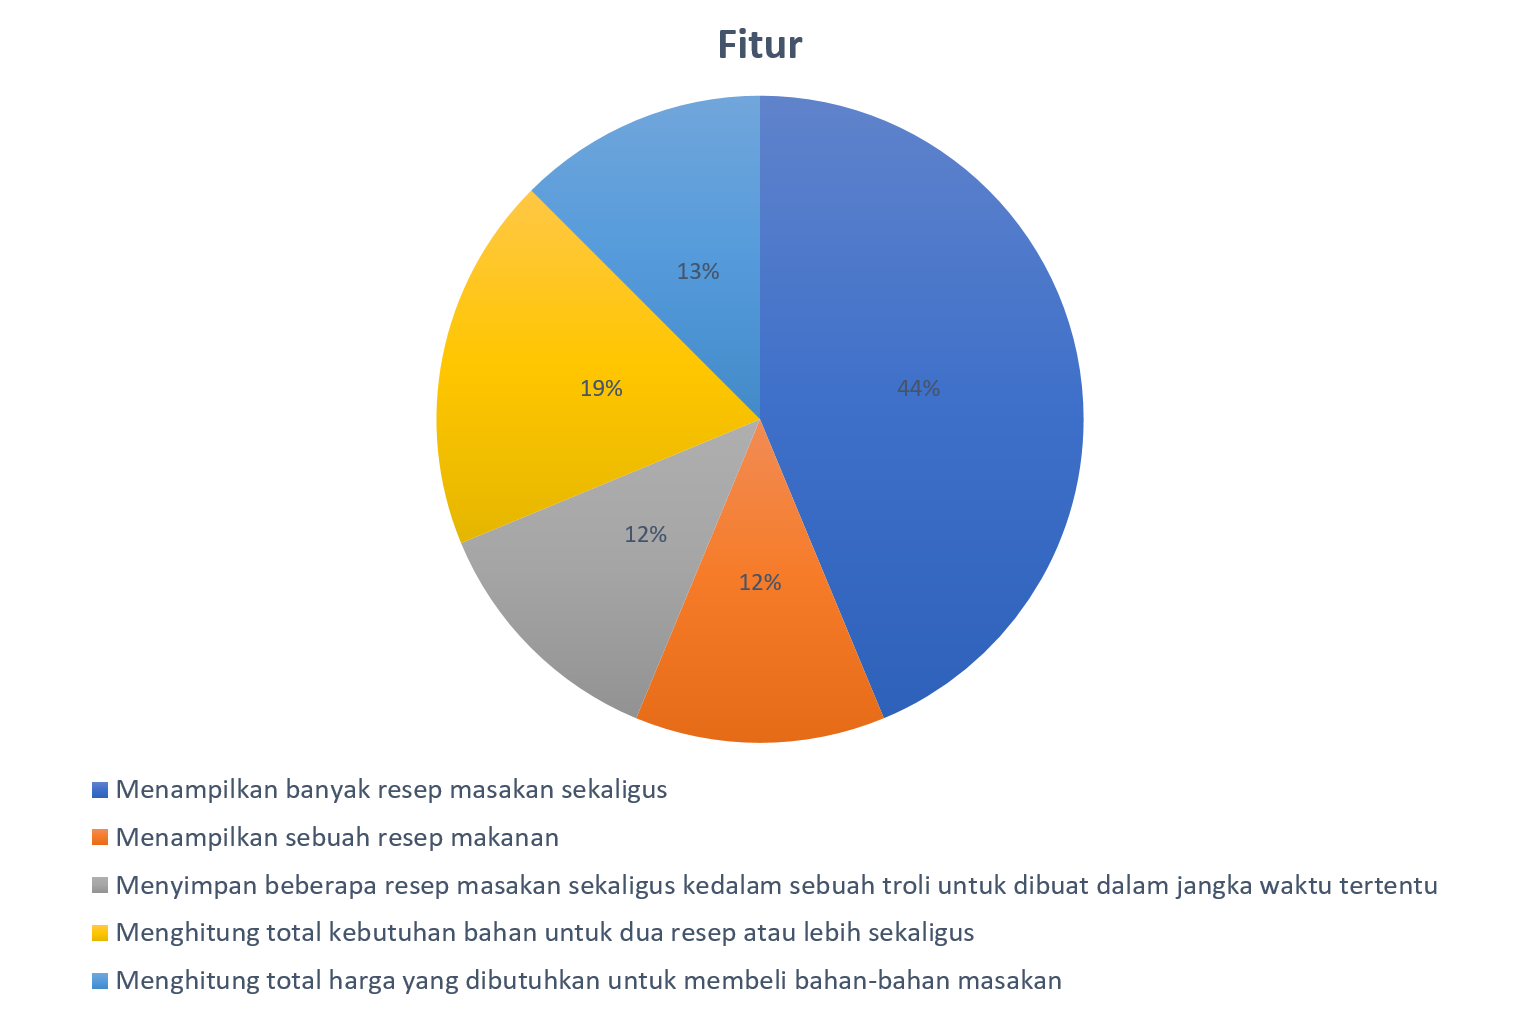
\includegraphics[width=1\textwidth]{gambar/pie/kuisioner_awam}
		\caption{\textit{Pie Chart} Hasil Kuisioner Awam}
	\end{figure}
	
	Masyarakat awam yang menjadi responden pada kuisioner yang telah disebar oleh Penulis menyertakan beberapa pendapat maupun ide tentang fitur apa yang seharusnya dimiliki oleh sebuah sistem aplikasi resep masakan berbasis Android, diantaranya adalah:
	\begin{itemize}
		\item Memberikan deskripsi bahan-bahan makanan yang dibutuhkan juga dan bisa didapatkan dimana
		\item Dalam sebuah resep akan lebih baik jika ada detail resep ini untuk berapa porsi, sehingga orang awam dapat mengetahui berapa takaran bahan-bahan masakan yang akan digunakan untuk porsi tertentu
		\item Menampilkan video tutorial masak, dan alternatif bahan masakan (bahan masakan pengganti untuk alergi misalnya)
		\item Aplikasi disertai video pembuatan masakan dan resepnya.	
	\end{itemize}
	
	Sedangkan dari usulan maupun ide yang datang dari para professional atau ahli di bidang ini adalah sebagai berikut:
	\begin{itemize}		
		\item Memberikan pilihan apa saja yang dapat dimasak dari suatu bahan-bahan tertentu
		\item Mengetahui kapan bahan akan habis
		\item Menampilkan metode memasak yang jelas sesuai dengan standar makanan yang akan dibuat
		\item Informasi jumlah takaran dalam sebuah resep haruslah jelas
		\item Mungkin bisa ditambah dengan foto atau video pembuatannya 
		\item Memberikan tips dan trik 
		\item Memberikan keterangan pada tulisan berbahasa asing untuk menambah pengetahuan. Contohnya \emph{Mise En Place} artinya preparasi
	\end{itemize}

	Melalui data yang telah terhimpun, penulis memutuskan untuk memilih fitur yang banyak dipilih oleh responden, baik ahli maupun kaum awam, untuk diimplemantasikan pada aplikasi yang akan dibuat oleh penulis, yaitu menampilkan banyak resep masakan sekaligus, menghitung total kebutuhan bahan untuk dua resep atau lebih sekaligus, menyimpan beberapa resep masakan sekaligus kedalam sebuah troli untuk dibuat dalam jangka waktu tertentu, serta menghitung total harga yang dibutuhkan untuk membeli bahan-bahan masakan. Sementara, fitur tambahan yang diinisiasi oleh penulis adalah fitur mencari resep berdasarkan bahan masakan yang akan dibuat.
	
\section{Desain}
	Dalam mengembangkan aplikasi ini, penulis mengembangkan desain aplikasi terlebih dahulu, mulai dari desain \emph{Use Case}, \emph{Entity Relationship Diagram} (ERD), \emph{Class Diagram}, serta \emph{Activity Diagram}. Selain itu, penulis juga membuat desain \textit{wireframe} dan \textit{mock-up}. Penulis memutuskan untuk membuat kedua desain tersebut untuk memudahkan pengguna dalam mengeksekusi desain antarmuka dari aplikasi ini. Berdasarkan pengalaman penulis dalam mengikuti program Praktek Kerja Lapangan pada PT Kompas Media Nusantara (Harian Kompas), dimana penulis berperan sebagai \textit{Front-End Developer}, perbedaan dari \textit{wireframe} dan \textit{mock-up} sendiri adalah pada tampilannya. Wireframe mengedepankan \textit{User Experience} dari sebuah laman aplikasi, yaitu alur kerja dari laman aplikasi tersebut. Biasanya tampilan yang disuguhkan oleh \textit{wireframe} tidak terlalu menarik dan hanya terlihat seperti kerangka dari tampilan aplikasi tersebut. 
	\begin{figure}[H]
		\centering
		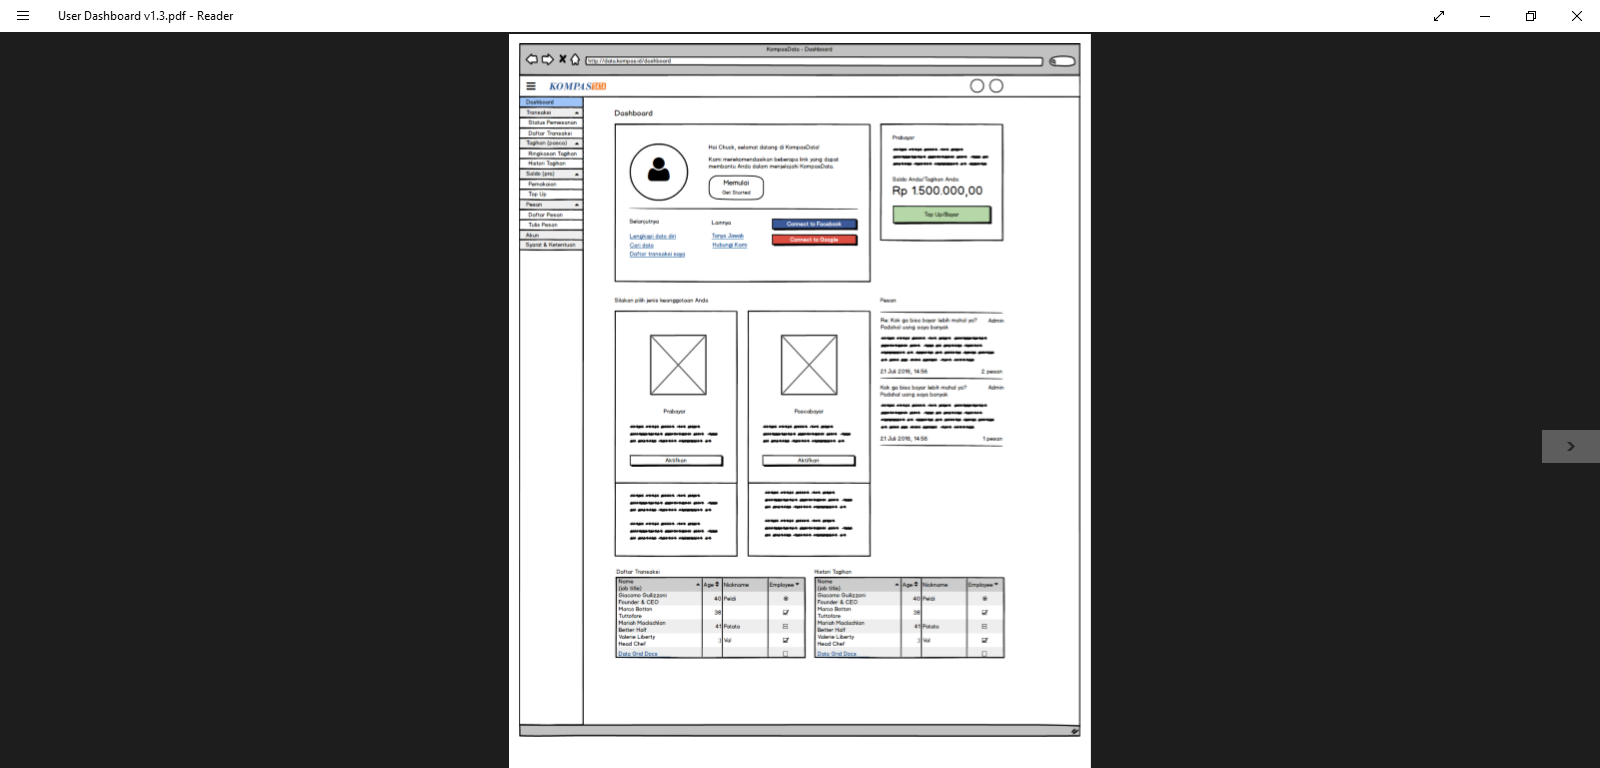
\includegraphics[origin=c,width=0.8\textwidth]{gambar/kompas/wireframe}
		\caption{Contoh \emph{Wireframe}}
		%\label{use case aplikasi}
	\end{figure}
	Sedangkan \textit{mock-up} adalah sebuah rancangan laman antarmuka aplikasi yang bersifat dekoratif dengan dekorasi yang sudah didefinisikan secara jelas oleh pembuatnya. \textit{Mock-up} menonjolkan sisi \textit{User Interface} dari sebuah laman antarmuka aplikasi. Berbeda dengan \textit{wireframe} yang hanya mengedepankan alur kerja dari sebuah laman, \textit{mock-up} adalah pengembangan lebih lanjut dari \textit{wireframe} sehingga sisi estetika dari sebuah rancangan antarmuka aplikasi lebih menonjol. \textit{Mock-up} memudahkan seorang Front-End Developer untuk mengembangkan dan mengeksekusi sebuah laman antarmuka aplikasi.
	\begin{figure}[H]
		\centering
		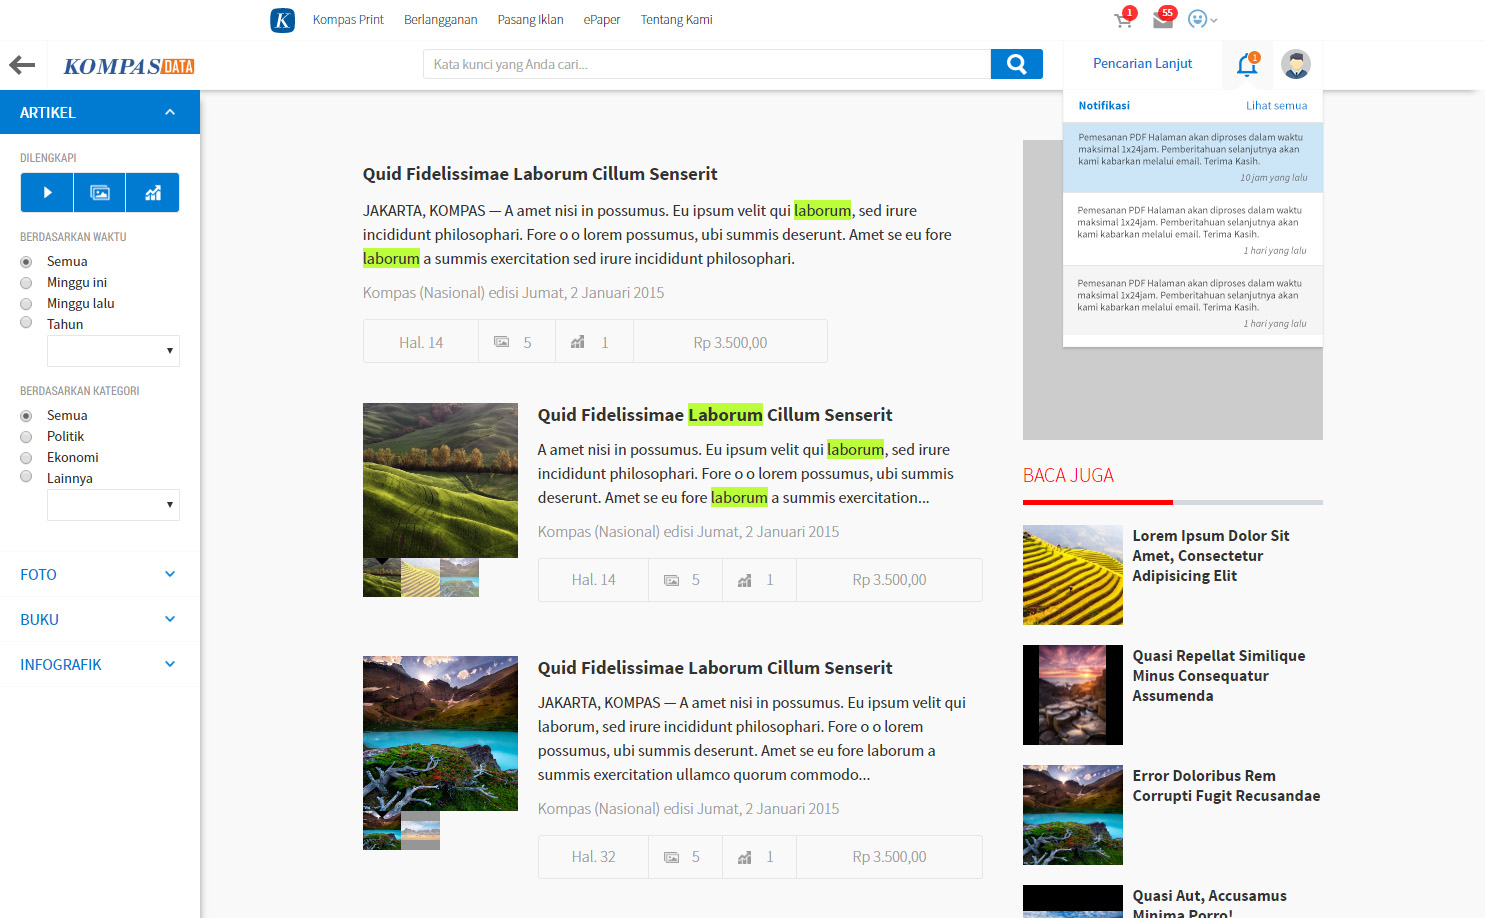
\includegraphics[origin=c,width=0.8\textwidth]{gambar/kompas/mock-up}
		\caption{Contoh \emph{Mock-Up}}
		%\label{use case aplikasi}
	\end{figure}
	 
	\subsection{\emph{Use Case Diagram}}
		\begin{figure}[H]
			\centering
			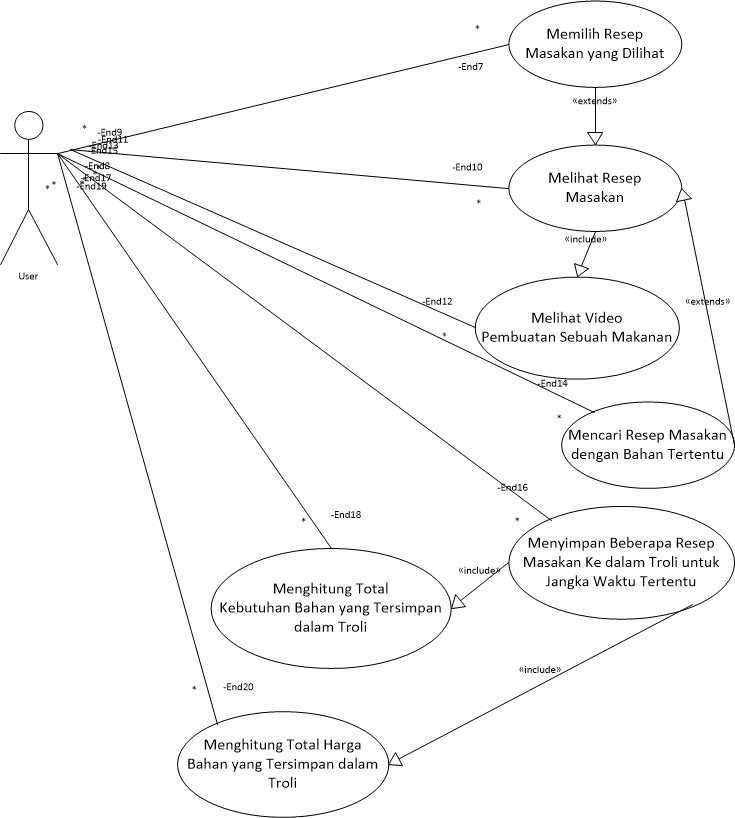
\includegraphics[origin=c,width=0.8\textwidth]{gambar/use-case/use_case_v2}
			%\caption{\emph{Use Case Diagram}}
			%\label{use case aplikasi}
		\end{figure}
		\textit{Use Case Diagram} tersebut menunjukkan bagaimana pengguna aplikasi (\textit{user}) berinteraksi dengan aplikasi yang dikembangkan oleh peneliti. Dalam \textit{use case} tersebut dijelaskan bahwa \textit{user} dapat memilih resep masakan yang ingin dilihat pada menu utama untuk kemudian melihat resep masakan sekaligus melihat video cara membuat makanan yang terdapat dalam resep tersebut. Selain itu, \textit{user} juga dapat mencari resep masakan berdasarkan bahan tertentu sesuai dengan keinginan \textit{user}. Setelah dilihat, \textit{user} dapat menyimpan resep masakan tersebut ke dalam Troli, dimana pada aplikasi ini disebut sebagai \textit{Wishlist}. \textit{User} dapat menyimpan sampai 3 resep masakan sekaligus dalam \textit{Wishlist}. Resep yang ada di dalam \textit{wishlist} dapat dihutung total kebutuhan bahannya dan juga dapat menghitung total kebutuhan harga untuk membeli bahan-bahan tersebut.   
	\subsection{\emph{Entity Relationship Diagram}}
		ERD pada aplikasi ini berfungsi untuk menyimpan resep, kategori resep, bahan-bahan yang ada  pada resep, cara memasak, serta harga pada tiap-tiap bahan yang tercantum dalam resep. Untuk itu, penulis membuat beberapa tabel untuk menunjang penyimpanan data dari tiap elemen tersebut. 
		
		\begin{figure}[H]
			\centering
			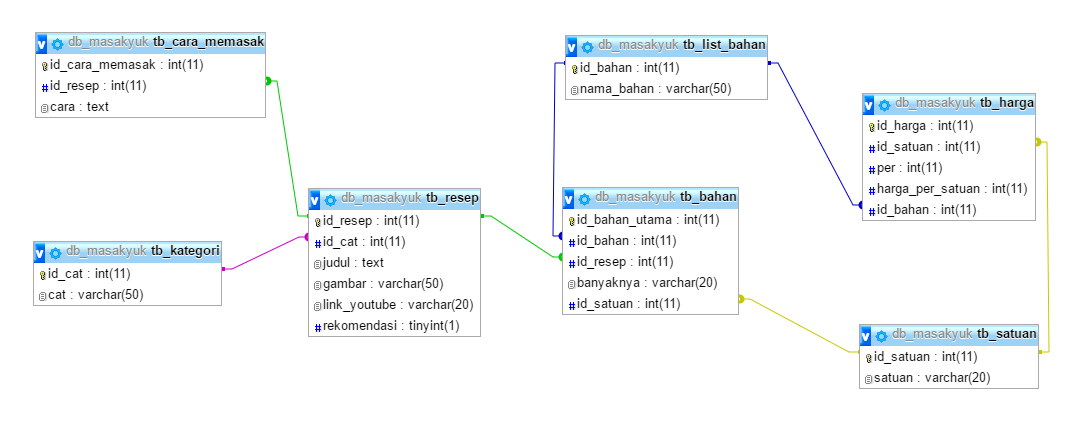
\includegraphics[width=1.1\textwidth]{gambar/erd_terbaru}
			\caption{\emph{Desain ERD Aplikasi yang Dikembangkan Penulis}}
			\label{erd_aplikasi}
			%angle=90,origin=c
		\end{figure}
		
		Penulis menyediakan tabel resep untuk menyimpan data-data yang berhubungan dengan resep. Kemudian, penulis juga menyediakan tabel bahan untuk menyimpan bahan-bahan yang terdapat pada sebuah resep serta tabel list atau daftar bahan untuk menyimpan data bahan-bahan secara umum yang dijadikan sebagai referensi dari tabel bahan. Penulis juga menyediakan tabel harga dan satuan untuk melengkapi tabel bahan. Tabel satuan dibuat karena adanya kemungkinan sebuah bahan dapat memiliki banyak jenis satuan, sedangkan tabel harga dibuat untuk menghitung harga bahan yang tertera dalam tabel bahan dengan kalkulasi yang berbeda bergantung pada satuannya. Selain itu, penulis juga membuat tabel cara memasak untuk menyimpan cara-cara memasak berdasarkan resep yang ada. Terakhir, penulis membuat tabel kategori untuk mengelompokkan rsep berdasarkan jenisnya yaitu Makanan Pembuka, Makanan Utama, dan Makanan Penutup.
		
		Tabel resep berelasi \textit{one-to-many} dengan tabel cara memasak dan tabel bahan karena satu resep dapat memiliki banyak cara memasak dan banyak bahan. Sedangkan tabel kategori berelasi \textit{one-to-many} juga karena satu kategori dapat memiliki banyak resep. Tabel list bahan berelasi \textit{one-to-many} dengan tabel bahan karena bahan yang terdapat pada tabel list bahan dapat dimasukkan lebih dari satu kali pada tabel bahan yang secara langsung menunjang tabel resep. Tabel Satuan berelasi one-to-many dengan tabel harga dan tabel bahan karena tabel harga dapat memiliki banyak satuan serta tabel bahan yang juga sama, yakni dapat memiliki lebih dari satu satuan.   
	\subsection{\emph{Class Diagram}}
		Pada pengembangan aplikasi resep masakan ini, penulis memecah \textit{class diagram} menjadi tiga bagian, yaitu \textit{class diagram} menu utama, \textit{class diagram} detail resep, dan \textit{class diagram wishlist}.
		
		Terdapat dua model yang diakses pada \textit{class diagram} Menu Utama. Resep Model digunakan untuk menyediakan data resep yang diolah pada \textit{controller} Resep Fragment, Rekomendasi Fragment, dan Jenis Fragment. Bahan Model digunakan untuk menyediakan data resep berdasarkan bahan yang dicari oleh \textit{user}.  \textit{Controller} selanjutnya mengalirkan data yang telah diolah kepada \textit{view} yang terdapat pada masing-masing \textit{controller}. Desain class diagram Mennu Utama dapat dilihat pada Gambar \ref{Class Diagram1}.  

		\begin{figure}[H]
			\centering
			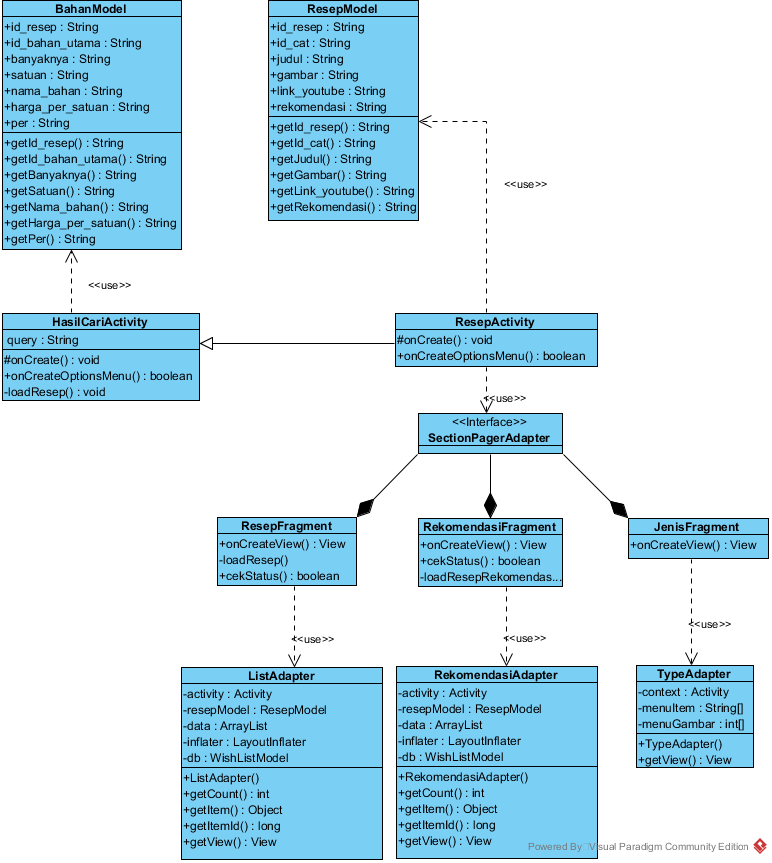
\includegraphics[origin=c,width=1\textwidth]{gambar/class/MenuUtama}
			\caption{\emph{Class Diagram} Menu Utama}
			\label{Class Diagram1}
		\end{figure}
		
		\textit{Class diagram} Detail Resep, yang terdapat pada Gambar \ref{Class Diagram Detail Resep}, memerlukan dua buah model yaitu Bahan Model dan Cara Model. Kedua model tersebut diperlukan untuk menyediakan data bahan yang dibutuhkan serta cara memasak dalam sebuah resep masakan. Data tersebut kemudian diolah dalam \textit{controller} BahanResepFragment dan CaraResepFragment untuk kemudian dialirkan kepada masing-masing \textit{view}
		
		\begin{figure}[H]
			\centering
			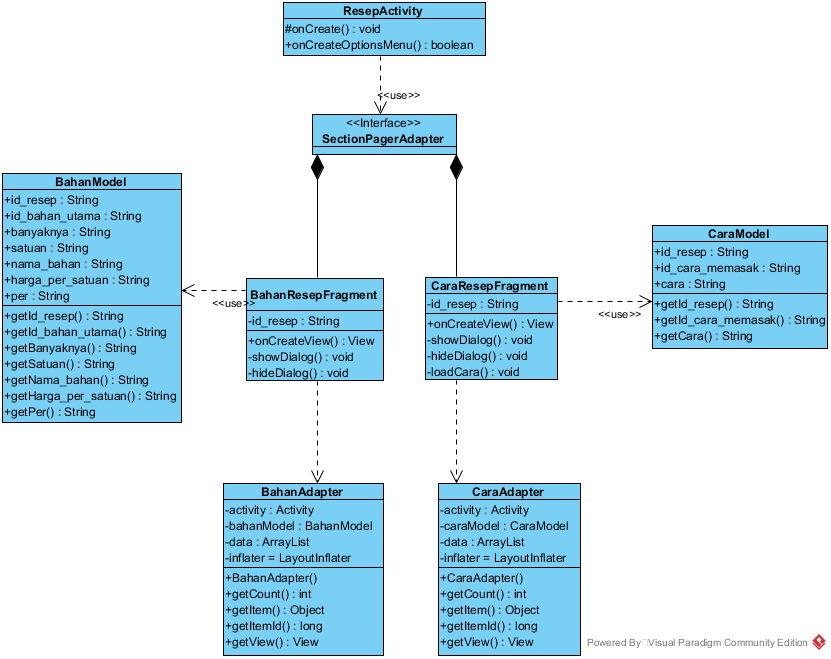
\includegraphics[origin=c,width=1\textwidth]{gambar/class/DetailResep}
			\caption{\emph{Class Diagram} Detail Resep}
			\label{Class Diagram Detail Resep}
		\end{figure}

		Wishlist merupakan \textit{class diagram} terakhir yag dibuat oleh penulis. Terdapat dua model yang digunakan dalam \textit{class diagram} ini yakni Bahan Model dan WishList Model. WishList Model digunakan untuk mengalirkan data resep yang telah disimpan oleh pengguna sebelumnya untuk kemudian dilakukan pencocokan data dengan basis data bahan (Bahan Model). Setelah dicocokkan, pengguna atau \textit{user} dapat melakukan perhitungan total bahan yang dibutuhkan serta melakukan perhitungan total harga bahan yang dibutuhkan oleh pengguna beserta dengan daftar harga tiap bahan yang dibutuhkan. Gambar \textit{class diagram wishlist} dapat dilihat pada Gambar \ref{Class wishlist}.
		
		\begin{figure}[H]
			\centering
			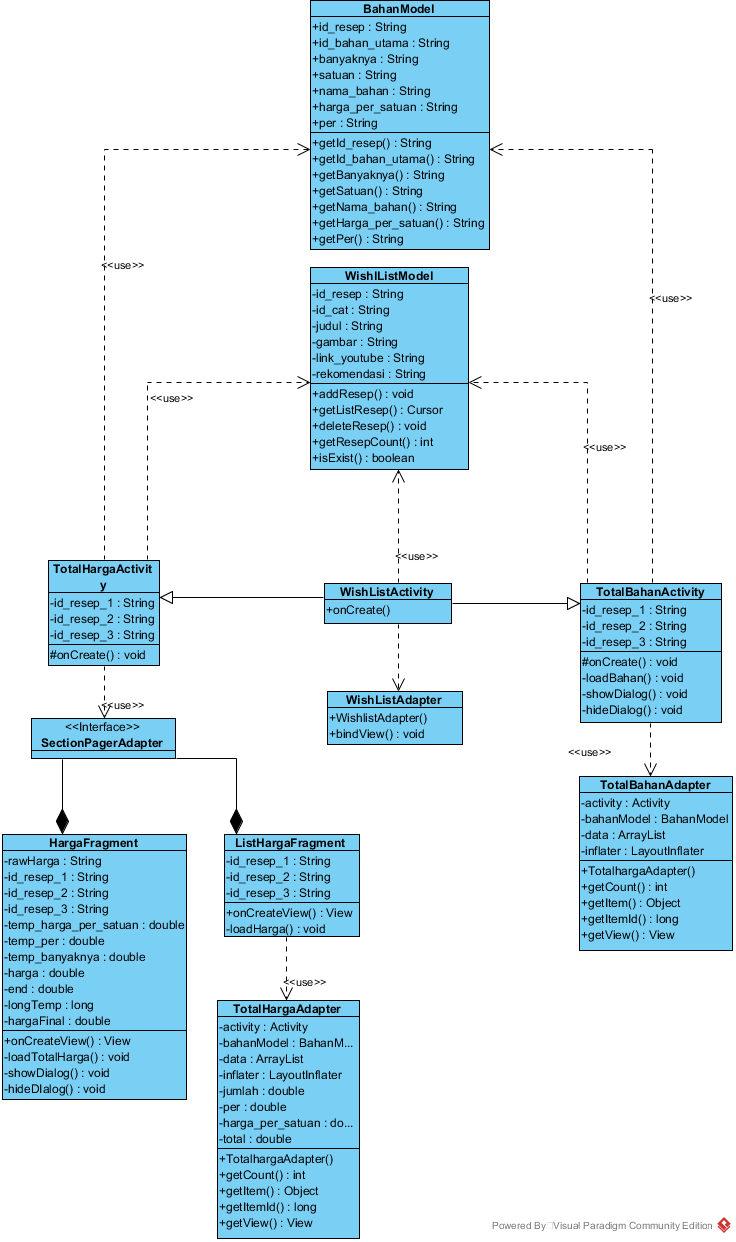
\includegraphics[origin=c,width=0.9\textwidth]{gambar/class/Wishlist}
			\caption{\emph{Class Diagram Wishlist}}
			\label{Class wishlist}
		\end{figure}

	\subsection{\emph{Activity Diagram}}
		Alur kerja aplikasi yang dikembangkan oleh penulis atau peneliti dapat dijelaskan melalui \textit{activity diagram} yang terdapat pada Gambar \ref{Activity Diagram1}
		\begin{figure}[H]
			\centering
			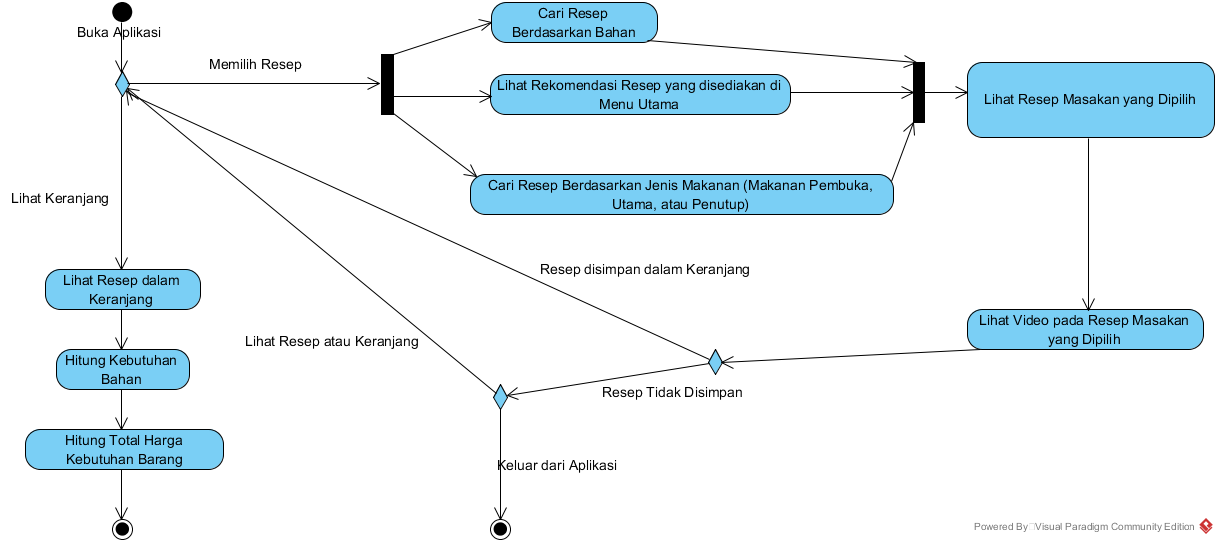
\includegraphics[origin=c,width=1\textwidth]{gambar/activity_diagram_v2}
			\caption{\emph{Activity Diagram dari Aplikasi yang Dibuat Penulis}}
			\label{Activity Diagram1}
		\end{figure}
		 Pada awal membuka aplikasi, pengguna aplikasi dapat memilih resep atau ingin melihat keranjang atau \textit{wishlist} apabila sudah pernah memasukkan resep ke dalam keranjang sebelumnya. Apabila pengguna ingin meilhat resep, maka pengguna dapat memilih resep dengan cara melihat daftar resep, mencari resep berdasarkan bahan, melihat rekomendasi resep yang disediakan, serta mencari resep berdasarkan jenis makanan (makanan pembuka, makanan utama, dan makanan penutup). Setelah itu, pengguna melihat resep yang telah dipilih serta dapat melihat video pembuatannya juga. Apabila resep disimpan kedalam keranjang, maka pengguna dapat kembali memilih resep atau melihat keranjang langsung untuk menghitung kebutuhan bahan serta total harga kebutuhan bahan. Sedangkan apabila resep masakan yang telah dilihat tidak dimasukkan ke dalam keranjang, maka pengguna dapat memilih resep masakan kembali, melihat keranjang yang sudah diisi sebelumnya, atau dapat keluar dari aplikasi.] 
	\subsection{Desain \textit{Wireframe} atau Kerangka Desain}
		\begin{figure}[H]
			\centering
			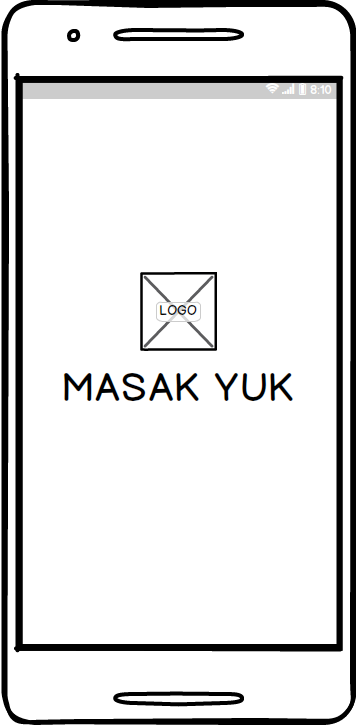
\includegraphics[width=0.25\textwidth]{gambar/wireframe/Splash}
			\caption{Halaman Awal}
			\label{splash}
		\end{figure}
		Desain halaman selamat datang ketika aplikasi pertama kali dimulai ditunjukkan pada Gambar \ref{splash}. Terdapat logo serta gambar latar belakang yang dibuat oleh penulis. Setelah tiga detik, pengguna akan diarahkan kepada laman utama aplikasi yang terdapat pada Gambar \ref{menu_utama} 
		\begin{figure}[H]
			\centering
			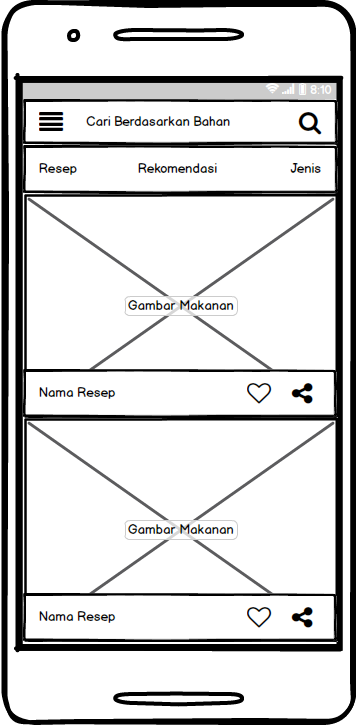
\includegraphics[width=0.25\textwidth]{gambar/wireframe/MenuUtama}
			\caption{Menu Utama}.
			\label{menu_utama} 
		\end{figure}
		Terdapat banyak resep masakan yang dapat dipilih pada laman ini. Pada laman menu utama, apabila pengguna mengusap layar dari rah kiri ke kanan, maka akan muncul menu navigasi seperti pada Gambar \ref{nav}. Pada menu navigasi, pengguna dapat memilih untuk melihat \textit{wishlist}, memberi masukan unuk aplikasi, membagikan aplikasi ke media sosial, dan keluar dari aplikasi
		\begin{figure}[H]
			\centering
			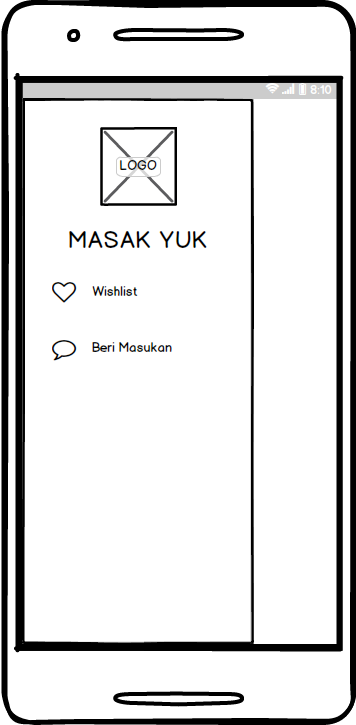
\includegraphics[width=0.25\textwidth]{gambar/wireframe/Drawer}
			\caption{Navigasi}
			\label{nav}
		\end{figure}
		Kembali lagi pada menu utama, apabila pengguna mengusap layar ke kanan atau menekan tab rekomendasi, maka akan muncul resep masakan yang direkomendasikan oleh aplikasi.
		\begin{figure}[H]
			\centering
			\includegraphics[width=0.25\textwidth]{gambar/wireframe/Rekomendasi}
			\caption{Menu Utama \textit{Tab} Rekomendasi}
		\end{figure}
		\vspace{2cm}
		Pada tab rekomendasi, apabila pengguna mengusap layar ke arah kanan, maka pengguna akan menemukan pilihan penampilan resep berdasarkan jenis makanannya yaitu makanan pembuka, makanan utama, dan makanan penutup.
		\begin{figure}[H]
			\centering
			\includegraphics[width=0.25\textwidth]{gambar/wireframe/Jenis}
			\caption{Menu Utama \textit{Tab} Jenis}
		\end{figure}
		Apabila pengguna memilih satu dari resep yang berada pada list yang disediakan dari menu-menu yang telah disebutkan sebelumnya, maka akan muncul laman detail resep yang terdiri dari video, bilah bahan resep serta bilah cara memasak dari resep tersebut
		\begin{figure}[H]
			\centering
			\includegraphics[width=0.25\textwidth]{gambar/wireframe/Resep}
			\caption{Detail Resep}
		\end{figure}
		Pengguna juga dapat melihat \textit{wishlist} dengan memanggil menu navigasi seperti pada Gambar \ref{nav} dan memilih menu \textit{wishlist}. Laman wishlist akan muncul seperti pada Gambar \ref{wire-wish}
		\begin{figure}[H]
			\centering
			\includegraphics[width=0.25\textwidth]{gambar/wireframe/Wishlist}
			\caption{Keranjang atau \textit{Wishlist}}
			\label{wire-wish}
		\end{figure}
		Pada laman \textit{wishlist}, pengguna dapat menghitung total bahan yang dibutuhkan untuk memasakn berdasarkkan resep yang telah dipilih dan ada pada keranjang
		\begin{figure}[H]
			\centering
			\includegraphics[width=0.25\textwidth]{gambar/wireframe/TotalBahan}
			\caption{Total Bahan}
		\end{figure}
		Selain itu, pada laman \textit{wishlist}, pengguna juga dapat menghitung total harga dari bahan-bahan dari resep yang telah masuk dalam \textit{wishlist}. 
		\begin{figure}[H]
			\centering
			\includegraphics[width=0.25\textwidth]{gambar/wireframe/TotalHarga}
			\caption{Total Harga}
		\end{figure}
	Pengguna juga dapat melihat rincian harga dari tiap bahan yang dibutuhkan oleh resep-resep yang terdapat pada \textit{wishlist}.
		\begin{figure}[H]
			\centering
			\includegraphics[width=0.25\textwidth]{gambar/wireframe/TotalHargaRincian}
			\caption{Rincian Total Harga}
		\end{figure}
	Kembali ke menu utama, pengguna juga dapat melakukan pencarian resep berdasarkan bahan yang dimiliki oleh pengguna.
		\begin{figure}[H]
			\centering
			\includegraphics[width=0.25\textwidth]{gambar/wireframe/HasilCari}
			\caption{Hasil Pencarian}
		\end{figure}
	Dan terakhir, desain \textit{wireframe} dari laman beri masukan yang dapat diakses melalui menu navigasi.	
		\begin{figure}[H]
			\centering
			\includegraphics[width=0.25\textwidth]{gambar/wireframe/BeriMasukan}
			\caption{Halaman Beri Masukan}
		\end{figure}
	\subsection{Desain \textit{Mock-Up} atau \textit{User Interface}}
		Setelah membuat wireframe, penulis kemudian langsung mengimplementasikan \textit{wireframe} tersebut ke dalam bentuk \textit{mock-up}. Dalam pengembangannya, \textit{mock-up} langsung dibuat dengan menggunakan xml sehingga mempercepat penulis dalam mengembangkan aplikasi resep masakan ini karena desain dari aplikasi tersebut sudah dikembangkan sekaligus dengan \textit{mock-up}. Selanjutnya penulis hanya perlu mengimplementasikan sistem \textit{Back-End} yang bekerja pada aplikasi resep masakan ini. Pengembangan \textit{mock-up} dapat dilihat pada Gambar \ref{mock-welcome} sampai Gambar \ref{mock-feedback}. Urutan pengembangan \textit{mock-up} sesuai dengan urutan pengembangan \textit{wireframe}.
		\begin{figure}[H]
			\centering
			\includegraphics[width=0.3\textwidth]{gambar/mock-up/splash}
			\caption{Halaman Awal atau Halaman Selamat Datang}
			\label{mock-welcome}
		\end{figure}
		\begin{figure}[H]
			\centering
			\includegraphics[width=0.3\textwidth]{gambar/mock-up/utama}
			\caption{Halaman Utama}
		\end{figure}
		\begin{figure}[H]
			\centering
			\includegraphics[width=0.3\textwidth]{gambar/mock-up/navigasi}
			\caption{Menu Navigasi}
		\end{figure}			
		\begin{figure}[H]
			\centering
			\includegraphics[width=0.3\textwidth]{gambar/mock-up/rekomendasi}
			\caption{Halaman Utama \textit{Tab} Rekomendasi}
		\end{figure}			
		\begin{figure}[H]
			\centering
			\includegraphics[width=0.3\textwidth]{gambar/mock-up/jenis}
			\caption{Halaman Utama \textit{Tab} Jenis}
		\end{figure}	
		\begin{figure}[H]
			\centering
			\includegraphics[width=0.3\textwidth]{gambar/mock-up/Detail}
			\caption{Detail Bahan Resep}
			\label{detail_bahan}
		\end{figure}
		\begin{figure}[H]
			\centering
			\includegraphics[width=0.3\textwidth]{gambar/mock-up/detail_cara}
			\caption{Detail Cara Memasak}
			\label{detail_cara}
		\end{figure}
		\begin{figure}[H]
			\centering
			\includegraphics[width=0.3\textwidth]{gambar/mock-up/wishlist}
			\caption{\textit{Wishlist}}
		\end{figure}
		\begin{figure}[H]
			\centering
			\includegraphics[width=0.3\textwidth]{gambar/mock-up/total_bahan}
			\caption{Total Bahan}
		\end{figure}	
		\begin{figure}[H]
			\centering
			\includegraphics[width=0.3\textwidth]{gambar/mock-up/total_harga}
			\caption{Total Harga}
		\end{figure}	
		\begin{figure}[H]
			\centering
			\includegraphics[width=0.3\textwidth]{gambar/mock-up/total_list_harga}
			\caption{Rincian Total Harga}
		\end{figure}	
		\begin{figure}[H]
			\centering
			\includegraphics[width=0.3\textwidth]{gambar/mock-up/cari_bahan}
			\caption{\textit{Tab} Pencarian}
		\end{figure}								
		\begin{figure}[H]
			\centering
			\includegraphics[width=0.3\textwidth]{gambar/mock-up/masukan}
			\caption{Laman Beri Masukan atau \textit{Feedback}}
			\label{mock-feedback}
		\end{figure}
				
\section{Konstruksi dan Pembangunan}
	Tahapan-tahapan dalam proses konstruksi dan pembangunan aplikasi berbasis resep masakan ini adalah sebagai berikut:
	\begin{enumerate}
		\item Membuat Basis Data
		\item Membuat API untuk Mengakses Basis Data
		\item Melakukan Input Data ke Basis Data
		\item Implementasi Desain Aplikasi
		\item Implementasi Metode Pertukaran Data antara Aplikasi dengan Basis Data
		\item Mengintegrasikan YouTube dengan Aplikasi Android
		\item Mengimplementasi Fitur Lainnya 
	\end{enumerate}

	\subsection{Membuat Basis Data}
		Basis data dibuat dengan menggunakan Basis Data MySQL atau MariaDB. Untuk mempercepat proses pengerjaan, penulis menggunakan aplikasi phpMyAdmin dalam membuat basis data secara keseluruhan, termasuk tabel dan entitas-entitas serta relasi yang terdapat di dalamnya. Basis data dibuat sesuai dengan ERD yang telah dibuat pada tahap desain.
		\begin{figure}[H]
			\centering
			\includegraphics[width=1\textwidth]{gambar/phpmyadmin_masakyuk}
			\caption{Basis Data yang Dibuat dengan phpMyAdmin}
			\label{phpmyadmin}
		\end{figure}
	
	\subsection{Membuat API untuk Mengakses Basis Data}
		Untuk dapat mengakses data yang terdapat pada basis data, dimana data tersebut tersimpan dalam server dengan jenis basis data MySQL atau MariaDB, maka penulis perlu membuat kumpulan API. Pengguna membuat API dengan menggunakan \textit{php framework} yaitu CodeIgniter. CodeIgniter mengimplementasi arsitektur Model-View-Controller dimana semua perintah menuju database secara langsung disimpan dalam Model dan mengolah data yang didapatkan oleh Model dengan menggunakan Controller. Data yang sudah dioleh kemudian ditampilkan melalui View.
		\begin{figure}[H]
			\centering
			\includegraphics[width=0.8\textwidth]{gambar/mvc-arch}
			\caption{Bagan Alur Kerja MVC}
			\label{mvc-3}
		\end{figure}
		Namun untuk membuat API, penulis tidak menggunakan View dari CodeIgniter tersebut. Penulis hanya pelu menyimpan \textit{query} basis data pada model dan API tersimpan dalam bagian Controller. Aplikasi Android nantinya akan mengakses Controller tersebut dan dijadikan sebagai API untuk mendapatkan akses kepada basis data. API yang dibuat untuk Aplikasi Android hanya memiliki metode yang bersifat \textit{read only}. Data akan diterima oleh aplikasi dalam bentuk JSON (JavaScript Object Notation).
		\begin{figure}[H]
			\centering
			\includegraphics[width=1\textwidth]{gambar/api/codeigniter_based_api}
			\caption{Bagan Alur Kerja CodeIgniter-Based API}
			\label{ci_based_api}
		\end{figure}
		Sampel kode dari CodeIgniter-Based API yang telah dibuat oleh Penulis dapat dilihat pada Gambar \ref{ci_sample_api} atau pada Lampiran C dan D.
		\begin{figure}[H]
			\centering
			\includegraphics[width=1\textwidth]{gambar/sample-api-ci}
			\caption{Sampel Kode CodeIgniter API-Based yang Dibuat Penulis}
			\label{ci_sample_api}
		\end{figure}
	
	\subsection{Melakukan Input Data ke Basis Data}
		Input data ke dalam \textit{database} dapat dilakukan dengan dua cara, yaitu memasukkan data melalui phpMyAdmin atau memasukan data melalui aplikasi web khusus untuk memasukkan data ke dalam basis data.
		\begin{figure}[H]
			\centering
			\includegraphics[width=1\textwidth]{gambar/insert-phpmyadmin}
			\caption{Input Data dengan phpMyAdmin}
			\label{insert_phpmyadmin}
		\end{figure} 
		Penulis mengembangkan aplikasi berbasis web dengan menggunakan \textit{framework} CodeIgniter yang khusus untuk memasukkan data ke dalam basis data. Adanya aplikasi berbasis web tersebut memudahkan penulis dalam memasukkan data-data ke dalam basis data, mulai dari data resep, bahan, hingga data harga bahan.
		\begin{figure}[H]
			\centering
			\includegraphics[width=1\textwidth]{gambar/web-list-resep}
			\caption{Tampilan List Resep pada Aplikasi Berbasis Web}
			\label{web-list-resep}
		\end{figure} 
		\begin{figure}[H]
			\centering
			\includegraphics[width=1\textwidth]{gambar/web-input-resep}
			\caption{Tampilan Input Resep pada Aplikasi Berbasis Web}
			\label{web-input-resep}
		\end{figure} 		
		Penulis melakukan sedikit modifikasi pada API yang telah dibuat dengan mengubah metode \textit{read only} menjadi \textit{read and write} dengan catatan yaitu write hanya diperbolehkan pada aplikasi berbasis web yang digunakan untuk memasukkan data-data yang dibutuhkan.  
		\begin{figure}[H]
			\centering
			\includegraphics[width=1\textwidth]{gambar/api/ci-api-web-chart}
			\caption{Bagan Alur Kerja CodeIgniter-Based API Hasil Modifikasi}
			\label{web-modification-resep}
		\end{figure} 	
	
	\subsection{Implementasi Desain Aplikasi}
		Desain Aplikasi sudah diimplementasikan kedalam bentuk \textit{layout} Android Studio yaitu dengan format xml sehingga penulis dapat melewati tahap implementasi desain ini. Implementasi dapat dilihat pada Bagian 3.2.6.
		
	\subsection{Implementasi Metode Pertukaran Data antara Aplikasi dengan Basis Data}
		Pada tahap ini, penulis mencoba mengimplementasikan API yang telah dibuat ke dalam aplikasi Android. Hal itu dilakukan agar aplikasi dapat melakukan pertukaran data dengan basis data dengan dijembatani oleh API yang telah dibuat sebelumnya. Pada aplikasi berbasis web, pertukaran data dilakukan dengan memanfaatkan Form GET/POST seperti pada Gambar \ref{req-html}.
		\begin{figure}[H]
			\centering
			\includegraphics[width=1\textwidth]{gambar/new/req_html}
			\caption{Bagan Alur Kerja Form GET/POST}
			\label{req-html}
		\end{figure}
		Dalam pengembangan aplikasi Android, salah satu cara untuk dapat memanggil CodeIgniter-Based API yang telah dibuat adalah dengan menggunakan Volley. Android Volley Library adalah sebuah \textit{library} yang disediakan oleh Google untuk dapat memfasilitasi akses \textit{Web-Based} API pada aplikasi Android sebagai media pertukaran data antara aplikasi dengan basis data. Cara Kerja Volley secara umum menyerupai Form GET/POST pada aplikasi berbasis web.
		\begin{figure}[H]
			\centering
			\includegraphics[width=1\textwidth]{gambar/new/req_volley}
			\caption{Bagan Alur Kerja Volley}
			\label{req-volley}
		\end{figure}
		Untuk dapat menggunakan Volley, penulis harus terlebih dahulu menambahkan compile 'com.android.volley:volley:1.0.0' pada berkas build.gradle yang terdapat di dalam direktori app.    	
	\subsection{Mengintegrasikan YouTube dengan Aplikasi Android}
		 Untuk dapat memainkan video YouTube pada aplikasi Android, maka dibutuhkan YouTube Android Player API sebagai perantara aplikasi dengan basis data YouTube. Penulis melakukan sedikit modifikasi pada implementasi YouTube Android Player API karena penggunaan Fragment pada Resep Activity. Ketika suatu \textit{class} pada Java Android Studio menggunakan Fragment, maka diperlukan \textit{class} yang melakukan ekstensi (\textit{extends}) dengan AppCompatActivity untuk mendukung pengelolaan beberapa Fragment yang akan ditampilkan pada sebuah Activity. Sedangkan YouTube Android Player API mewajibkan penggunanya untuk melakukan ekstensi terhadap \textit{class} YouTubeBaseActivity
 		\begin{figure}[H]
		 	\centering
		 	\includegraphics[width=1\textwidth]{gambar/new/youtube_player_view}
		 	\caption{Bagan Alur Kerja YouTubePlayerView pada sebuah Activity}
		 	\label{youtube-player-view}
		 \end{figure}
		\vspace{1cm}
		Apabila Activity tetap mengekstensi YouTubeBaseActivity, maka Activity tersebut tidak dapat mengelola Fragment yang terdapat didalamnya karena kehilangan metode getSupportFragmentManager() yang berasal dari ekstensi \textit{class} terhadap AppCompatActivity. Maka dari itu, penulis melakukan modifikasi dengan tidak menggunakan YouTubePlayerView, melainkan menggunakan YouTubePlayerFragment. Keputusan tersebut diambil karena YouTubePlayerFragment "lebih ramah" terhadap Activity yang memiliki Fragment dengan tidak perlu mengekstensi \textit{class} YouTubeBaseActivity sehingga seluruh Fragment yang ada pada sebuah Activity dapat dikelola dengan baik. Perbedaannya adalah seluruh metode yang diberikan oleh YouTube Android Player API tidak dilakukan \textit{override}, melainkan langsung diinisialisasikan pada metode onCreate sebuah Activity. 
 		\begin{figure}[H]
			\centering
			\includegraphics[width=1\textwidth]{gambar/new/youtube_player_fragment}
			\caption{Bagan Alur Kerja YouTubePlayerFragment pada sebuah Activity}
			\label{youtube-player-frag}
		\end{figure}
		\vspace{1cm}
		Sampel kode implementasi YouTubePlayerFragment terdapat pada Gambar \ref{youtube-frag-sampel}.
 		\begin{figure}[H]
			\centering
			\includegraphics[width=1\textwidth]{gambar/new/youtube_fragment}
			\caption{Sampel Kode Implementasi YouTubePlayerFragment pada Metode onCreate sebuah Activity}
			\label{youtube-frag-sampel}
		\end{figure}
	\subsection{Mengimplementasi Fitur Lainnya}
		Fitur lain yang diimplementasikan oleh penulis adalah fitur penyimpanan \textit{wishlist}, menghitung total bahan pada resep yang terdapat dalam \textit{wishlist}, menghitung total harga bahan yang terdapat pada \textit{wishlist} dan menampilkan rincian harga per bahan. \textit{Wishlist} sendiri dibuat dengan memanfaatkan basis data SQLite dengan menggunakan bahasa query yang sama yakni SQL. Basis data SQLite bersifat lokal dan terdapat didalam aplikasi itu sendiri. Jadi, apabila pengguna aplikasi menghapus data aplikasi pada ponselnya, maka data \textit{wishlist} pun juga akan hilang.
		
		Wishlist mampu menampung maksimal tiga resep masakan. Untuk dapat menghitung total bahan dan total harga bahan yang terdapat pada resep-resep tersebut, maka data yang terdapat di dalam SQLite dikirimkan dan diolah oleh API yang telah dibuat untuk kemudian disalurkan kembali hasil perhitungannya pada aplikasi. Alur dari proses penyimpanan pada \textit{wishlist} hingga perhitungan total bahan dan harga bahan dijelaskan pada Gambar \ref{fitur-lain}
		\begin{figure}[H]
			\centering
			\includegraphics[width=1\textwidth]{gambar/new/fitur_lain}
			\caption{Alur Penyimpanan pada SQLite dan Pengolahan Total Bahan dan Harga Bahan}
			\label{fitur-lain}
		\end{figure}

%!TEX root = ./template-skripsi.tex
%-------------------------------------------------------------------------------
%                            BAB IV
%               		HASIL DAN PEMBAHASAN
%-------------------------------------------------------------------------------

\chapter{UJI COBA DAN HASIL UJI COBA}
	\section{Uji Coba}
		Dalam proses pengembangan aplikasi sesuai dengan SDLC, khususnya SDLC model spiral, uji coba dapat dikategorikan sebagai proses Evaluasi. Aplikasi yang telah selesai dikembangkan kemudian diujicobakan oleh beberapa ahli sebelum nantinya dirilis untuk masyarakat luas. Ahli yang akan menilai aplikasi ini adalah tiga dari empat ahli yang telah mengisi kuisioner identifikasi pada saat penelitian ini dimulai. Penulis mendatangi ketiga responden tersebut untuk melakukan uji coba dengan menggunakan ponsel milik penulis. Pertanyaan yang diajukan untuk para ahli berkisar tentang ketepatan dan kesesuaian konten yang dihasilkan oleh aplikasi. Komponen yang dinilai pada Uji Ahli tersebut adalah:
		\begin{itemize}
			\item Penilaian Konten Aplikasi
			\begin{enumerate}
				\item List Bahan yang tampil sesuai dengan resepnya
				\item List Cara Memasak yang tampil sesuai dengan resepnya
				\item Video YouTube yang diputar sesuai dengan Resepnya
				\item Takaran bahan tepat
				\item Langkah-langkah memasak yang ditampilkan tepat
			\end{enumerate}
			\item Penilaian Tampilan Aplikasi
			\begin{enumerate}
				\item Tulisan dapat dibaca dengan baik
				\item Elemen-elemen dalam aplikasi tertata dengan baik
				\item Ukuran gambar ideal (tidak terlalu besar atau kecil)
				\item Perpindahan antar halaman lancar
				\item Video YouTube dapat diputar dengan baik
				\item Wishlist dapat ditampilkan dengan baik
				\item Total Bahan pada Wishlist dapat ditampilkan dengan baik
				\item Total Harga pada Wishlist dapat ditampilkan dengan baik
				\item Total Rincian Harga pada Wishlist dapat ditampilkan dengan baik
			\end{enumerate}
			\item Penilaian Fungsionalitas Aplikasi
			\begin{enumerate}
				\item Resep dapat dimasukkan ke dalam Wishlist
				\item Resep dapat dihapus dari Wishlist
				\item Fitur Pencarian dapat mencari sesuai Bahan Resep
				\item Resep dapat dibagikan ke media sosial
			\end{enumerate}
		\end{itemize}
	
		Semua komponen penilaian tersebut akan dinilai dengan \textit{range} nilai antara 1 sampai 5 dengan perincian sebagai berikut:
		\begin{itemize}
			\item Nilai 1 - Sangat tidak setuju
			\item Nilai 2 - Tidak setuju
			\item Nilai 3 - Cukup
			\item Nilai 4 - Setuju
			\item Nilai 5 - Sangat setuju
		\end{itemize}
		\vspace{5cm}
		Data yang telah diperoleh kemudian dikalkulasikan dengan menggunakan sistem penilaian sebagai berikut:
		\begin{itemize}
			\item Nilai total\\
			Nilai ini adalah nilaitotal dari tiap pernyataan. Nilai total ini didapat dengan menggunakan persamaan sebagai berikut:\\
			$Nilai$ $total$ $=$ $jumlah$ $nilai$ $tiap$ $soal$
			\item Nilai rata-rata\\
			Nilai ini adalah nilai rata-rata dari tiap pernyataan dan didapat dengan menggunakan persamaan:\\
			$Nilai  rata-rata = \frac{nilai total}{jumlah partisipan}$
		\end{itemize}
	
	\section{Hasil Uji Coba Berdasarkan Aspek Penilaian}		
		Setelah dilakukan uji coba oleh tiga ahli di bidang kuliner dengan 18 item penilaian yang diajukan dengan sebaran 5 item penilaian konten, 9 item penilaian tampilan, dan 4 item penilaian fungsionalitas, penulis mengolah data hasil penilaian dari para ahli. Hasil diolah berdasarkan aspek penilaian yakni konten, tampilan, dan fungsionalitas.
		
		\subsection{Hasil Uji Coba Konten}
		
			\begin{table}[H]
				\centering
				\includegraphics[width=0.6\textwidth]{gambar/new/konten_tabel}
				\caption{Tabel Nilai Hasil Uji Coba Konten}
				\label{tabel_konten}
			\end{table}
			Tabel \ref{tabel_konten} menunjukkan bahwa item penilaian ketiga, yakni Video YouTube yang diputar sesuai dengan resepnya, memiliki nilai tertinggi yaitu 5. Selanjutnya item penilaian kedua, yaitu list cara Memasak yang tampil sesuai dengan resepnya, menempati peringkat kedua dengan nilai 4,67. Item penilaian yang menempati peringkat ketiga dan keempat secara berturut-turut adalah item penilaian kelima dan pertama (langkah-langkah/cara-cara memasak yang ditampilkan tepat dan list bahan yang tampil sesuai dengan resepnya). Item penilaian dengan nilai terendah ditempati oleh item penilaian keempat dengan nilai 3 yakni takaran bahan tepat.  

		\subsection{Hasil Uji Coba Tampilan}

			\begin{table}[H]
				\centering
				\includegraphics[width=1\textwidth]{gambar/new/tampilan_tabel}
				\caption{Tabel Nilai Hasil Uji Coba Tampilan}
				\label{tabel_tampilan}
			\end{table}
			Tabel \ref{tabel_tampilan} menunjukkan bahwa item penilaian kelima, yakni video YouTube dapat dimainkan dengan baik, memiliki nilai tertinggi yaitu 5. Sedangkan item penilaian kedua, yakni elemen-elemen dalam aplikasi tertata dengan baik, menempati posisi terbawah dengan nilai 3,33.
	
		\subsection{Hasil Uji Coba Tampilan}

			\begin{table}[H]
				\centering
				\includegraphics[width=0.6\textwidth]{gambar/new/fungsi_tabel}
				\caption{Tabel Nilai Hasil Uji Coba Fungsionalitas}
				\label{tabel_fungsionalitas}
			\end{table}
			Tabel \ref{tabel_fungsionalitas} menunjukkan bahwa item penilaian ketiga, yakni fitur pencarian dapat mencari sesuai bahan resep, dan item penilaian keempat, yakni resep dapat dibagikan ke media sosial, masing-masing memiliki nilai tertinggi yaitu 5. Sedangkan item penilaian pertama dan kedua, yakni resep dapat dimasukkan ke dalam \textit{wishlist} dan resep dapat dihapus dari \textit{wishlist}, masing-masing memiliki nilai terendah dengan nilai 4,67.			
	
	\section{Hasil Uji Coba Secara Keseluruhan}
		Dari data-data uji coba yang telah diolah berdasarkan aspek penilaian, dari segi konten, video YouTube yang diputar sesuai dengan resepnya, menempati peringkat teratas dalam proses uji coba. Dari segi tampilan, item penilaian video YouTube dapat dimainkan dengan baik juga menempati peringkat teratas. Sedangkan dari segi fungsionalitas, fitur pencarian dapat mencari sesuai bahan resep serta resep dapat dibagikan ke media sosial masing-masing juga menempati peringkat teratas. Hal ini menunjukkan bahwa video YouTube telah berhasil diimplementasikan secara baik dari segi konten maupun tampilan. Sedangkan fitur lain yang dapat berfungsi secara baik adalah fitur pencarian resep berdasarkan bahan serta fitur \textit{sharing} resep ke media sosial. Sejauh ini dapat disimpulkan bahwa implementasi YouTube kedalam aplikasi Android telah berhasil dilakukan.
		
		Sementara itu, para ahli juga memberikan beberapa masukkan kepada penulis untuk pengembangan aplikasi selanjutnya, yaitu:
		\begin{enumerate}
			\item Akan lebih baik apabila tampilan pada aplikasi ini tertata lebih baik lagi. Fungsi mencari bahan pada aplikasi ini sangat baik.
			\item Tambahkan fitur kapan bahan yang dimasak akan habis. 
			\item Kembangkan juga aplikasi untuk dapur restoran khususnya \textit{storing} bahan baku yang mencatat stok bahan di dapur.
			\item Berikan jumlah takaran yang lebih jelas lagi (beberapa bahan seperti gula dan garam tidak diberikan takaran yang spesifik)
			\item Berikan tips dan trik dalam memasak resep tersebut
			\item Memberikan keterangan pada tulisan berbahasa asing untuk menambah pengetahuan (contoh sudah diberikan pada kuisioner awal) 
		\end{enumerate} 
		
% Baris ini digunakan untuk membantu dalam melakukan sitasi.
% Karena diapit dengan comment, maka baris ini akan diabaikan
% oleh compiler LaTeX.
\begin{comment}
\bibliography{daftar-pustaka}
\end{comment}

%!TEX root = ./template-skripsi.tex
%-------------------------------------------------------------------------------
%                            	BAB V
%               		KESIMPULAN DAN SARAN
%-------------------------------------------------------------------------------

\chapter{KESIMPULAN DAN SARAN}

\section{Kesimpulan}
	Berdasarkan hasil implementasi dan pengujian konten, tampilan, serta fungsionalitas aplikasi ini, didapat kesimpulan sebagai berikut:

	\begin{enumerate}
		\item Bentuk aplikasi kumpulan resep masakan terintegrasi \textit{food channel} YouTube dapat dilihat pada Gambar \ref{mock-welcome} - Gambar \ref{mock-feedback}. Bentuk spesifik dimana \textit{food channel} YouTube diletakkan pada aplikasi tersebut terdapat pada Gambar \ref{detail_bahan} dan Gambar \ref{detail_cara}.
		
		\item Aplikasi kumpulan resep masakan terintegrasi \textit{food channel} YouTube dikembangkan dengan mengacu pada \textit{System Development Life Cycle} (SDLC) model Spiral dengan tahapan yaitu Identifikasi, Desain, Konstrusi dan Pembangunan, dan yang terakhir adalah Evaluasi.
		
		\item YouTube dapat diintegrasikan dengan aplikasi Android dengan menggunakan YouTube Android Player API. Penggunaan API YouTube tersebut disesuaikan dengan kebutuhannya dalam sebuah antarmuka aplikasi Android. Apabila digunakan pada Activity utuh maka dapat digunakan YouTubePlayerView. Sedangkan jika menggunakan Activity yang terdiri dari satu atau lebih Fragment, maka digunakan YouTubePlayerFragment. 

		\item Berdasarkan hasil uji coba, dapat disimpulkan bahwa \textit{food channel} YouTube berhasil diimplementasikan pada aplikasi yang dikembangkan oleh penulis. Hal tersebut ditunjukkan dengan item penilaian video YouTube dapat dimainkan dengan baik juga menempati peringkat teratas dalam segi tampilan serta video YouTube yang diputar sesuai dengan resepnya, menempati peringkat teratas dalam proses uji coba dari segi konten. Fitur-fitur lainnya turut melengkapi aplikasi resep masakan terintegrasi \textit{food channel} YouTube ini. Dengan kata lain, aplikasi ini berhasil diuji dengan baik dan siap dirilis ke masyarakat luas. 
	\end{enumerate}


\section{Saran}
	Adapun saran-saran penulis untuk penelitian selanjutnya adalah:
	\begin{enumerate}
		\item Menambahkan informasi bagaimana cara memasak yang baik dan benar sesuai dengan standar yang berlaku dalam dunia memasak serta menambah kosakata bahasa asing maupun bahasa daerah untuk memperkaya pengetahuan pengguna aplikasi. 
		
		\item Menambah kapasitas \textit{wishlist} menjadi lebih dari 3.
		
		\item Membuat aplikasi yang dapat menjangkau lebih banyak versi Android, termasuk versi Android sebelum API 21 atau Android 5.0 (Lollipop). 
		
		\item Membuat aplikasi kumpulan resep masakan yang mampu memuat lebih dari satu video pada setiap resepnya.
		
		\item Menggunakan basis data Firebase sebagai pengganti SQL karena Firebase juga merupakan produk Google sama dengan Android. Banyak kemampuan yang mampu dimaksimalkan dengan penggunaan Firebase sebagai basis data dari sebuah aplikasi Android.
		
		\item Jika masih mengembangkan dengan menggunakan CodeIgniter-Based API ataupun API berbasis \textit{web framework} lainnya, penggunaan Retrofit menggantikan Volley sangat disarankan karena kecepatan akses data yang jauh lebih cepat daripada Volley. 

	\end{enumerate}

	
% Baris ini digunakan untuk membantu dalam melakukan sitasi
% Karena diapit dengan comment, maka baris ini akan diabaikan
% oleh compiler LaTeX.
\begin{comment}
\bibliography{daftar-pustaka}
\end{comment}

%-----------------------------------------------------------------
%Disini akhir masukan Bab
%-----------------------------------------------------------------


%-----------------------------------------------------------------
% Disini awal masukan untuk Daftar Pustaka
% - Daftar pustaka diambil dari file .bib yang ada pada folder ini
%   juga.
% - Untuk memudahkan dalam memanajemen dan menggenerate file .bib
%   gunakan reference manager seperti Mendeley, Zotero, EndNote,
%   dll.
%-----------------------------------------------------------------
%\bibliography{IEEEabrv,daftar-pustaka}
\begin{thebibliography}{99}
	\bibitem{anisya}Anisya. 2013. "Aplikasi Sistem Database Rumah Sakit Terpusat pada Rumah Sakit Umum (RSU) Aisyiyah Padang dengan Menerapkan Open Source (PHP - MySQL)". Jurnal Momentum.

	\bibitem{tutorialspoint} Artikel non-personal.  2016. "SDLC - Spiral Model".  Tutorials Point [Online]. Tersedia: \url{https://www.tutorialspoint.com/sdlc/sdlc_spiral_model.htm}. [28 Oktober 2016].
	
	\bibitem{bagui}Bagui, Sikha dan Richard Earp. 2011. \textit{Database Design Using Entity-Relationship Diagram}. Florida: CRC Press.	
	
	\bibitem{bell} Bell, Donald.  2003. "An Introduction to the Unified Modeling Language".  IBM developerWorks [Online]. Tersedia: \url{http://www.ibm.com/developerworks/rational/library/769.html}. [01 November 2016].
	
	\bibitem{burton}Burton, Michael dan Donn Felker. 2012. \textit{Android Application Development For Dummies, 2nd Edition}. New Jersey: John Wiley and Sons, Inc.	
	
	\bibitem{denis}Denis, Alan, Barbara Haley Wixom dan David Tegarden. 2010. \textit{Systems Analysis and Design with UML: An Object-Oriented Approach 3rd Edition}. New Jersey: John Wiley and Sons, Inc.
	
	\bibitem{edi} Edi, Doro dan Stevalin Betshani. 2009. "Analisis Data dengan Menggunakan ERD dan Model Konseptual Data Warehouse". Jurnal Informatika, Vol.5, No. 1, Juni 2009.
	
	\bibitem{francis} Francis, Danny. 2013. "Perancangan Aplikasi Customer Relationship Management: Studi Kasus PT Primacipta Megah Jaya". Thesis Magister pada FASILKOM Universitas Indonesia.

	\bibitem{lee} Lee, Sunguk. 2012. "Unified Modeling Language (UML) for Database Systems and Computer Application". International Journal of Database Theory and Application.
	
	\bibitem{murtiwiyati} Murtiwiyati dan Glenn Lauren. 2013. "Rancang Bangun Aplikasi Pembelajaran Budaya Indonesia Untuk Anak Sekolah Dasar Berbasis Android". Jurnal Ilmiah KOMPUTASI, Volume 12 Nomor : 2, Desember 2013.	

	\bibitem{myers} Myers, Brad A dan Jeffrey Stylos. 2016. "Improving API Usability". Communications of the ACM, vol 59, No. 6, June, 2016.		
	
	\bibitem{palupi}Palupi, Sri dan Tuti Hera Widi Handayani. 2010. \textit{Resep Masakan (Modul 2)}. Yogyakarta: Universitas Negeri Yogyakarta.	
	
	\bibitem{inirani} Pertiwi, Ratih Sukma dan Annelis Brillian.  2015. "Perempuan, Mari Kembali ke Dapur!".  Tabloid Nova [Online]. Tersedia: \url{http://tabloidnova.com/Sedap/Tips-Masak/Perempuan-Mari-Kembali-Ke-Dapur}. [28 April 2016].	
	
	\bibitem{pressman}Pressman, Roger S. 2010. \textit{Software Engineering A Practitioner's Approach}. New York: McGraw Hill.	
		
	\bibitem{rogers}Rogers, Rick, dkk. 2009. \textit{Android Application Development}. California: O'Reilly Media.	
	
	\bibitem{poernomo} Setyanti, Christina Andhika dan Syafrina Syaaf.  2014. "3 Alasan Utama Perempuan Malas Masak".  Kompas.com [Online]. Tersedia: \url{http://female.kompas.com/read/2014/03/06/1254310/3.Alasan.Utama.Perempuan.Malas.Masak}. [28 April 2016].
	
	\bibitem{soenardi}Soenardi, Tuti dan Tim. 2013. \textit{Teori Dasar Kuliner}. Jakarta: PT Gramedia Pustaka Utama.	
		
	
\end{thebibliography}
\addcontentsline{toc}{chapter}{DAFTAR PUSTAKA}
%-----------------------------------------------------------------
%Disini akhir masukan Daftar Pustaka
%-----------------------------------------------------------------
\appendix{} 
\addcontentsline{toc}{chapter}{LAMPIRAN}
\includepdf[pages=1, scale=0.6, pagecommand={\chapter{Hasil Kuisioner Identifikasi oleh Ahli}}]{pdf/identifikasi_ahli.pdf}
\includepdf[pages=2-, scale=0.6]{pdf/identifikasi_ahli.pdf}

\includepdf[pages=1, scale=0.6, pagecommand={\chapter{Hasil Kuisioner Identifikasi oleh Awam}}]{pdf/identifikasi_masyarakat.pdf}
\includepdf[pages=2-, scale=0.6]{pdf/identifikasi_masyarakat.pdf}


\chapter{Sampel API Buatan Penulis Bagian Model}
	\begin{verbatim}
		function get_resep(){
			$obj = $this->db->select('*')
							->get('tb_resep');
			return $obj->result_array();
		}
		
		function get_list_bahan($id_resep){
			$obj = $this->db->select('*')
							->join('tb_list_bahan',
							'tb_list_bahan.id_bahan = tb_bahan.id_bahan')
							->join('tb_satuan',
							'tb_satuan.id_satuan = tb_bahan.id_satuan')
							->where('id_resep',$id_resep)
							->get('tb_bahan');
			return $obj->result_array();
		}
		
		function get_list_cara($id_resep){
			$obj = $this->db->select('*')
						->where('id_resep',$id_resep)
						->get('tb_cara_memasak');
			return $obj->result_array();
		}
		
		function get_search_bahan($query){
			$obj = $this->db->select('*')
							->join('tb_kategori',
							'tb_kategori.id_cat = tb_resep.id_cat')
							->join('tb_bahan',
							'tb_bahan.id_resep = tb_resep.id_resep')
							->join('tb_list_bahan',
							'tb_list_bahan.id_bahan = tb_bahan.id_bahan')
							->like('nama_bahan',$query)
							->get('tb_resep');
			return $obj->result_array();
		}
		
	\end{verbatim}	
\chapter{Sampel API Buatan Penulis Bagian Controller}
	\begin{verbatim}
		function get_resep(){
			$query = $this->Masakyuk_model->get_resep();
			$response = array();
			$cek = $query;
			if($cek > 0){
				$response["resep"]	=array();
				foreach ($query as $row) {
					$data=array();
					$data["id_resep"]		=	$row["id_resep"];
					$data["id_cat"]	=	$row["id_cat"];
					$data["judul"]	=	$row["judul"];
					$data["gambar"]	=	$row["gambar"];
					$data["link_youtube"]	=	$row["link_youtube"];
					$data["rekomendasi"]	=	$row["rekomendasi"];
					array_push($response["resep"], $data);
				}
				$response["success"]	= 1;
				$response["message"]	= "Semua data resep";
				echo json_encode($response);
			} else {
				$response["success"]	= 0;
				$response["message"]	= "Data resep tidak ditemukan";
				echo json_encode($response);
			}
		}
		
		function get_list_bahan_resep(){
			if($this->input->post('id_resep')){
				$id_resep=$this->input->post('id_resep');
			}
			$query = $this->Masakyuk_model->get_list_bahan($id_resep);
			$response = array();
			$cek = $query;
			if($cek > 0){
				$response["bahan"]	=array();
				foreach ($query as $row) {
					$data=array();
					$data["id_resep"]		=	$row["id_resep"];
					$data["id_bahan_utama"]		=	$row["id_bahan_utama"];
					$data["banyaknya"]	=	$row["banyaknya"];
					$data["satuan"]	=	$row["satuan"];
					$data["nama_bahan"]	=	$row["nama_bahan"];
					array_push($response["bahan"], $data);
				}
				$response["success"]	= 1;
				$response["message"]	= "Semua data bahan";
				echo json_encode($response);
			} else {
				$response["success"]	= 0;
				$response["message"]	= "Data bahan tidak ditemukan";
				echo json_encode($response);
			}
		}
		
		function get_list_cara_memasak(){
			if($this->input->post('id_resep')){
				$id_resep=$this->input->post('id_resep');
			}
			$query = $this->Masakyuk_model->get_list_cara($id_resep);
			$response = array();
			$cek = $query;
			if($cek > 0){
				$response["cara"]	=array();
				foreach ($query as $row) {
					$data=array();
					$data["id_resep"]		=	$row["id_resep"];
					$data["id_cara_memasak"]		=	$row["id_cara_memasak"];
					$data["cara"]	=	$row["cara"];
					array_push($response["cara"], $data);
				}
				$response["success"]	= 1;
				$response["message"]	= "Semua cara memasak resep";
				echo json_encode($response);
			} else {
				$response["success"]	= 0;
				$response["message"]	= "Data cara memasak tidak ditemukan";
				echo json_encode($response);
			}
		}
		
		function get_list_hasil_cari(){
			\indif($this->input->post('query')){
				$query=$this->input->post('query');
			}
			$query = $this->Masakyuk_model->get_search_bahan($query);
			$response = array();
			$cek = $query;
			if($cek > 0){
				$response["resep"]	=array();
				foreach ($query as $row) {
					$data=array();
					$data["id_resep"]		=	$row["id_resep"];
					$data["id_cat"]	=	$row["id_cat"];
					$data["cat"]	=	$row["cat"];
					$data["judul"]	=	$row["judul"];
					$data["gambar"]	=	$row["gambar"];
					$data["link_youtube"]	=	$row["link_youtube"];
					$data["rekomendasi"]	=	$row["rekomendasi"];
					array_push($response["resep"], $data);
				}
				$response["success"]	= 1;
				$response["message"]	= "Semua data resep";
				echo json_encode($response);
			} else {
				$response["success"]	= 0;
				$response["message"]	= "Data resep tidak ditemukan";
				echo json_encode($response);
			}
		}		
	\end{verbatim}	

\includepdf[pages=1, scale=0.6, pagecommand={\chapter{Hasil Kuisioner Uji Coba Ahli}}]{pdf/hasil_uji_ahli.pdf}
\includepdf[pages=2-, scale=0.6]{pdf/hasil_uji_ahli.pdf}


\end{document}